%%%%%%%%%%%%%%%%%%%%%%%%%%%%%%%%%%%%%%%%%%%%%%%%%%%%%%%%%%%%%%%%%%%%%%%
%
% Presentation of Beamer UMN Theme
% Beamer Presentation by Tambe E. Norbert of UMN--Twin Cities
% Hacked From Chris Bourke of Univ Nebraska--Lincoln
% June 13th, 2014
%
%%%%%%%%%%%%%%%%%%%%%%%%%%%%%%%%%%%%%%%%%%%%%%%%%%%%%%%%%%%%%%%%%%%%%%%
\documentclass{beamer}
\usetheme[hideothersubsections,hideallsubsections]{UMNTheme}
% Remove navigation symbols
\setbeamertemplate{navigation symbols}{}
\title{Search For Delayed Photons Using Timing.}
%\subtitle{}
\author[Tambe E. Norbert] % (optional, for multiple authors)
{Shih-Chuan Kao\inst{1} \and Yuichi Kubota\inst{1} \and Tambe E. Norbert\inst{1} \and Roger Rusack\inst{1}}
\institute[UMN]{
\inst{1}%
University Of Minnesota
}
\vspace{-2cm}
\date{ Long-Lived Meeting,\\ \today}
\begin{document}
%{% open a Local TeX Group
%\setbeamertemplate{sidebar}{}
\begin{frame}
\titlepage
\begin{center}
\href{mailto:norbe072@umn.edu}{\color{cyan}{\texttt{norbert@physics.umn.edu.edu}}}
\end{center}
\end{frame}
%}% end Local TeX Group
\section*{Outline}
\begin{frame}
\frametitle{\Huge Outline}
\tableofcontents
\end{frame}

%%% Intro for General Talks
\begin{frame}
\frametitle{\huge{Where are we now?}}
\begin{varblock}[7cm]{\textbf{The Universe Set}}
 The set  $S =\{ \cdots \mathbf{0}, \frac{1}{2}, 1,  \frac{3}{2}, 2  \cdots \} \cdot \hbar $ 
 \end{varblock}
 where $s$ is the spin of a particle. 
 represents our past, current and probably future understanding of the universe around us. As of the moment 
Currently we know:
 \begin{itemize}
  \item $\mathbf{s = \frac{1}{2}\hbar}$ Describes all the matter in our universe.
  \item $\mathbf{s = 1\hbar}$ Describes gauge interactions.
  \item $\mathbf{s = 0\hbar}$ Responsible for giving mass.
  \item $\mathbf{s = 2\hbar}$ Describes gravity~(gauged?).
  \item $\mathbf{s = \frac{3}{2}\hbar}$ \textcolor{red}{?? \textbf{Dark Matter}?}
 \end{itemize}

However, this magic set only describes $\approx 4$\% of our total universe.
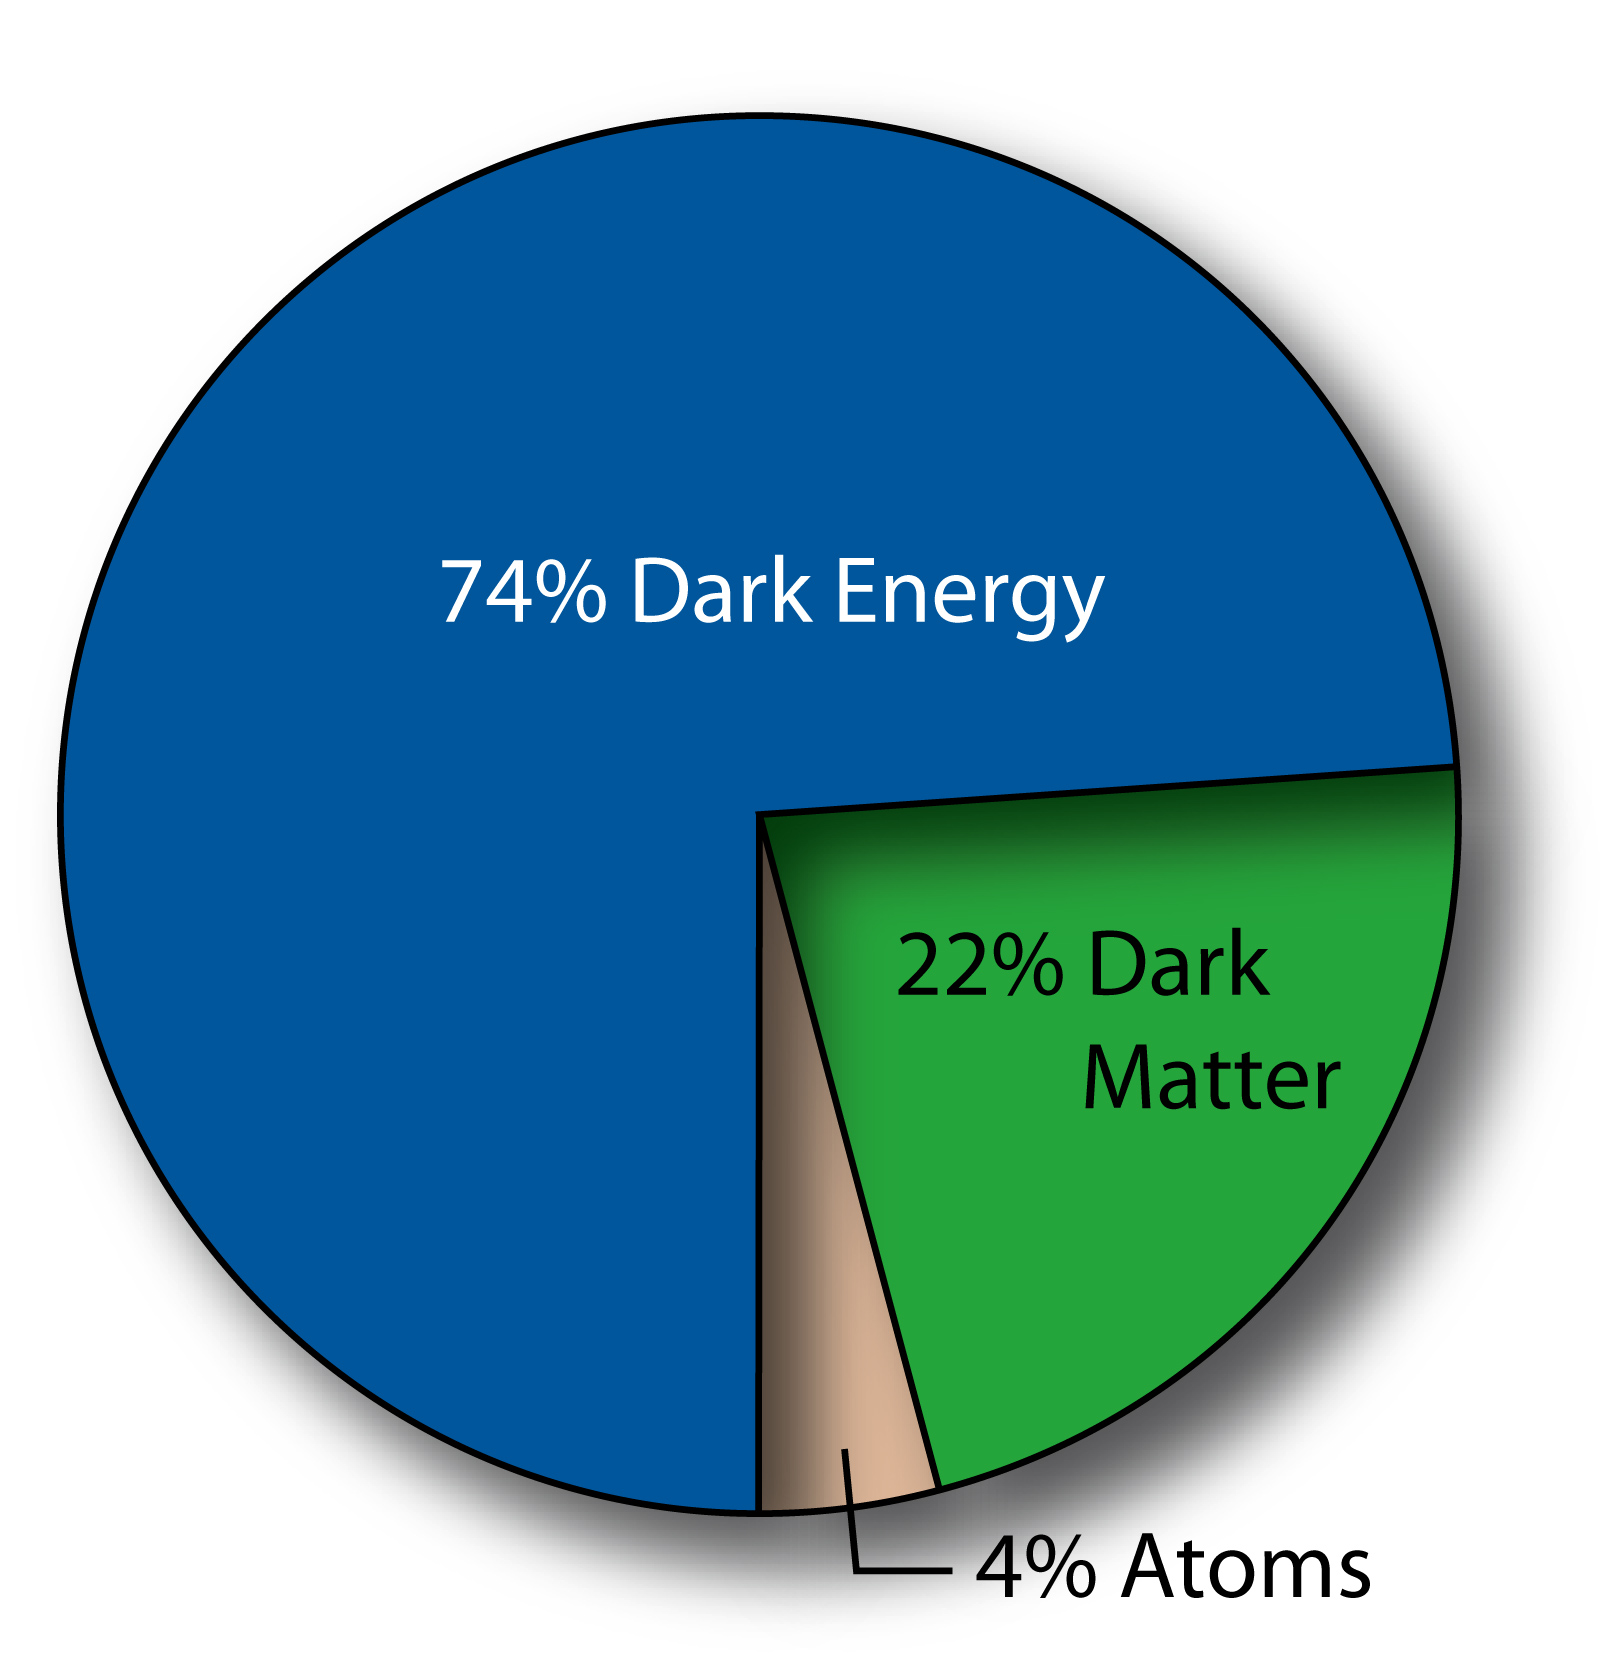
\includegraphics[height=2cm,width=0.25\paperwidth]{THESISPLOTS/UniversePie30.jpg}
\end{frame}



%% For Pre-Approval talk Intro Page
\section{Introduction}
\begin{frame}
% \tableofcontents
% \framesubtitle{}
% \vspace{-1cm}
\frametitle{\Huge Introduction}

\frametitle{\Huge Introduction}
 %\vspace{-0.5cm}
\begin{minipage}{0.8\paperwidth} 
     \begin{itemize}  
       \item{\color{UMN@Maroon} \textbf{Long-Lived Particle Models}}
      \large{
       \setbeamertemplate{itemize items}{$\mathbb{\star}$}
        \begin{itemize}
        \item Gauge Mediated Supersymmetry Breaking~(GMSB)
        \setbeamertemplate{itemize items}{$\mathbb{\triangleright}$}
          \begin{itemize}
            \item Next-to-lightest SUSY~(NLSP) is \alert{Neutralino}~($\tilde{\chi}^{0}_{1}$)
            \item $eV-keV$ Lightest-SUSY particle~(LSP) is \textcolor{blue}{Gravitino}~($\tilde{G}$).
            \item Gravitino is a Dark Matter Candidate.
          \end{itemize}
        \setbeamertemplate{itemize items}{$\mathbb{\star}$}  
        \item General Gauge Mediation~(GGM)
         \setbeamertemplate{itemize items}{$\mathbb{\triangleright}$}
          \begin{itemize}
            \item NLSP is a mixture of fermions~(Bino, Wino, Higssino).
            \item Several SUSY particles can be NLSP.
          \end{itemize}
      \end{itemize}
    }   
  \item{ \color{UMN@Maroon} \textbf{ECAL Resolution}}    
 %\end{itemize}
%\end{minipage}%

%\begin{minipage}[b]{0.8\paperwidth}
  \begin{columns}
    \begin{column}{0.5\textwidth} 
     %%% Left Column
      %\vspace{-1cm}
      %\fboxsep=0pt  
       %\fbox{%
      % \begin{itemize}
       % \item{ \color{UMN@Maroon} \textbf{ECAL Timing}}
       \setbeamertemplate{itemize items}{$\mathbb{\dagger}$} %\otimes, \ominus etc
           \begin{itemize}
             \item ECAL timing resolution $\sigma_{t} < 500$~ps.
             \item Use timing to identify photons and electrons from long-lived decay.
           \end{itemize}
      % \end{itemize}                 
     \end{column}% 
% Right Column
     % \hspace{0.5cm}
     \begin{column}{0.6\textwidth}
       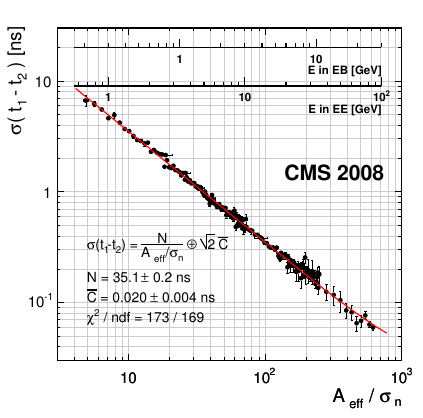
\includegraphics[width=0.75\textwidth]{THESISPLOTS/ECAL_Timing_Resolution.png}        
     \end{column} 
   \end{columns} 
     
  \end{itemize}
\end{minipage}
 
\end{frame}

%% SUSY at LHC
\begin{frame}
\frametitle{LHC Supersymmetry Production}
 % \begin{tikzpicture}[remember picture,overlay]
 %     \node[at=(current page.center)] {
 %     \includegraphics[width=\paperwidth]{THESISPLOTS/SUSY-XSEC.pdf}
 %           };
 %  \end{tikzpicture}
% \usebackgroundtemplate{\includegraphics[width=\paperwidth]{THESISPLOTS/SUSY-XSEC.pdf}}
 \begin{minipage}[t]{0.5\linewidth}
   \includegraphics[height=7cm,width=0.45\paperwidth]{THESISPLOTS/SUSY-XSEC.pdf}
   %\caption{}
   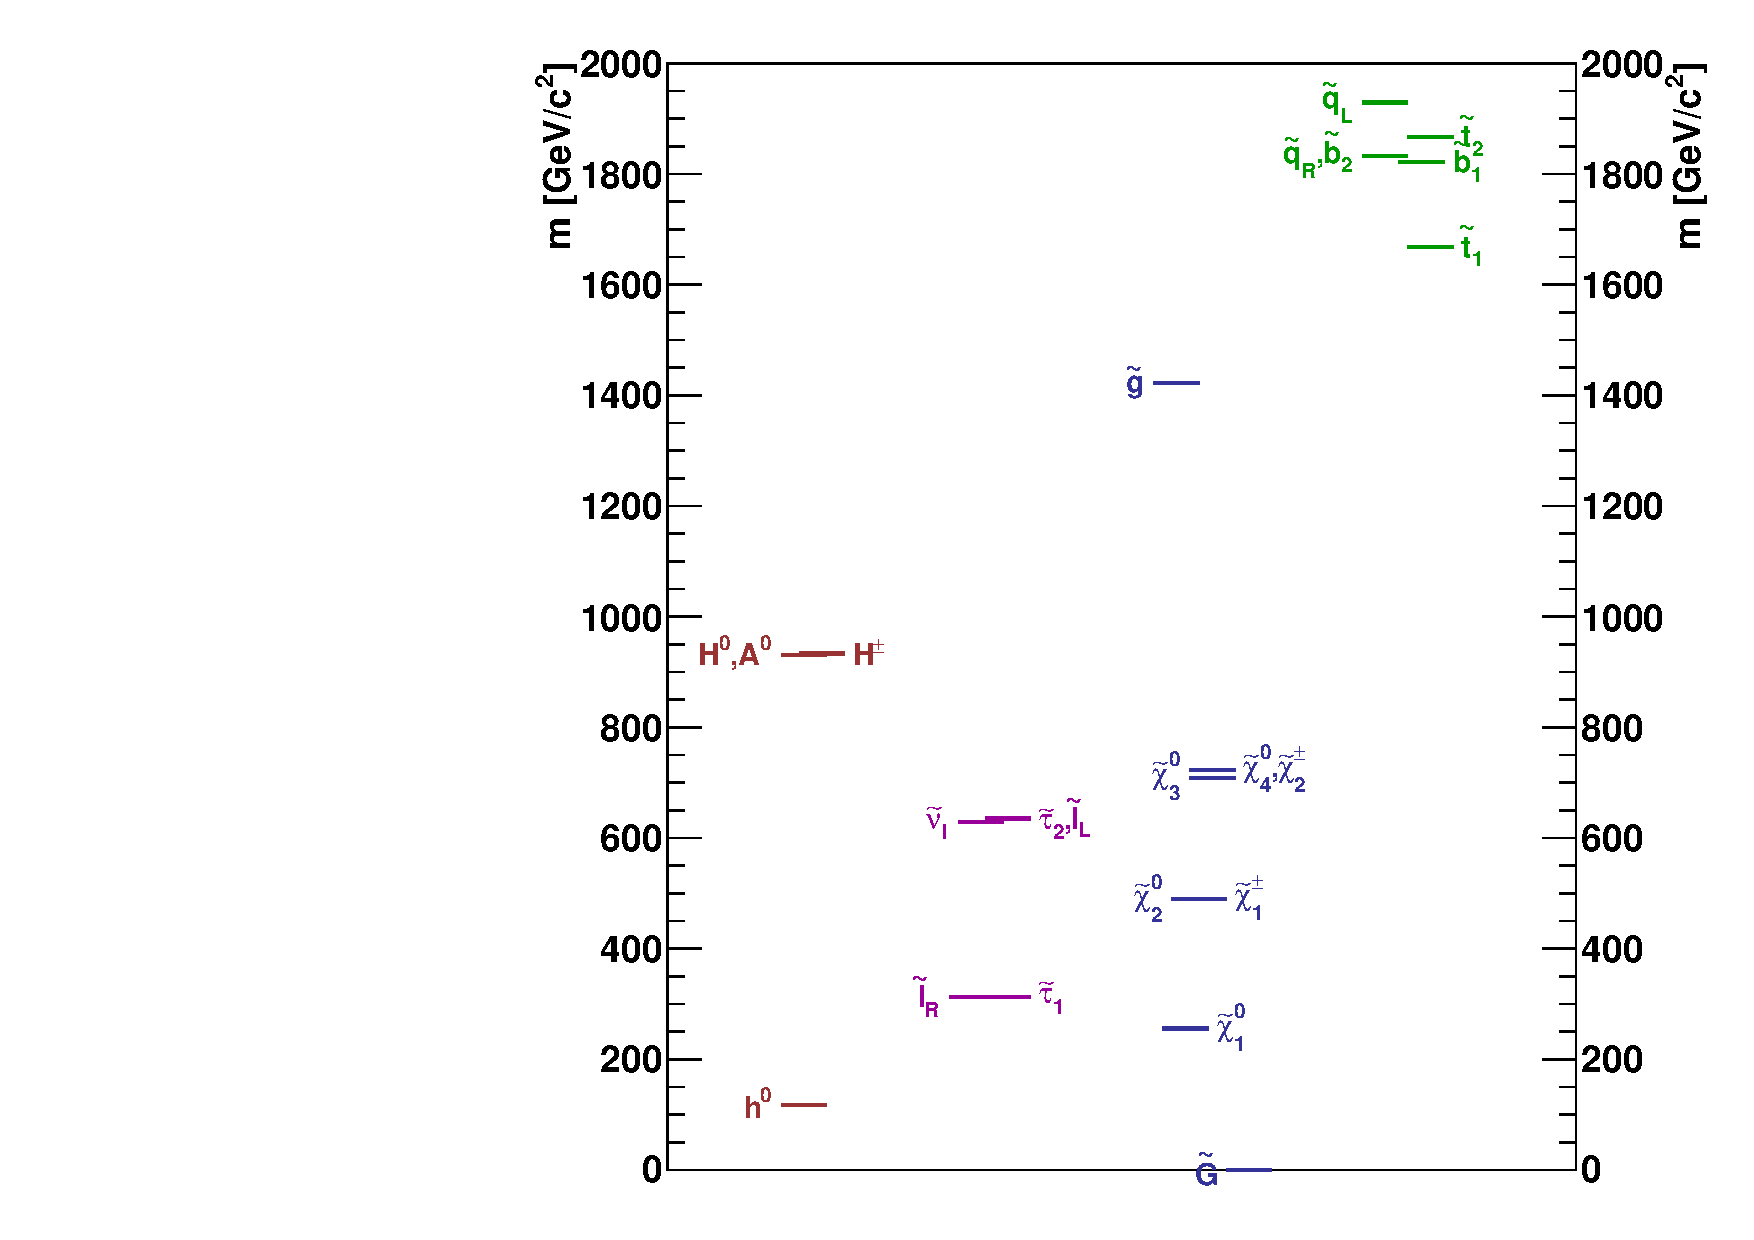
\includegraphics[height=6.5cm,width=0.40\paperwidth]{THESISPLOTS/gmsb_Lambda180_CTau10000.pdf}
 \end{minipage} 
 %\caption{mGMSB:SPS8 model}
   
 \begin{minipage}[b]{\linewidth}
   SUSY production mostly in strong interactions at LHC.
 \end{minipage}
\end{frame}

%% Production and Decay
\section{Production and Decay}
\begin{frame}
\frametitle{\Huge Cascade Decay Chain}
 %\begin{columns}
 % \begin{column}{1.\textwidth}
   \begin{minipage}[t]{0.7\linewidth}
 %    \centering
      \includegraphics[width=0.80\paperwidth]{THESISPLOTS/SUSY-DECAY.pdf}
 \end{minipage}
 %\begin{minipage}[b]{0.7\linewidth}
 \newline \textcolor{blue} {\texttt{Y. Kats et al: arXiv:1110.6444v2}}
 %\end{minipage}
    
\end{frame}    
\begin{frame}
\frametitle{Delayed Photon Production}   
  %  \hspace{5cm}
   % \begin{minipage}[t]{0.5\paperwidth}
 %     \centering 
  \fboxsep=0pt  
  \begin{varblock}[7cm]{Double Photon}
  % \fbox{%
   \centering
    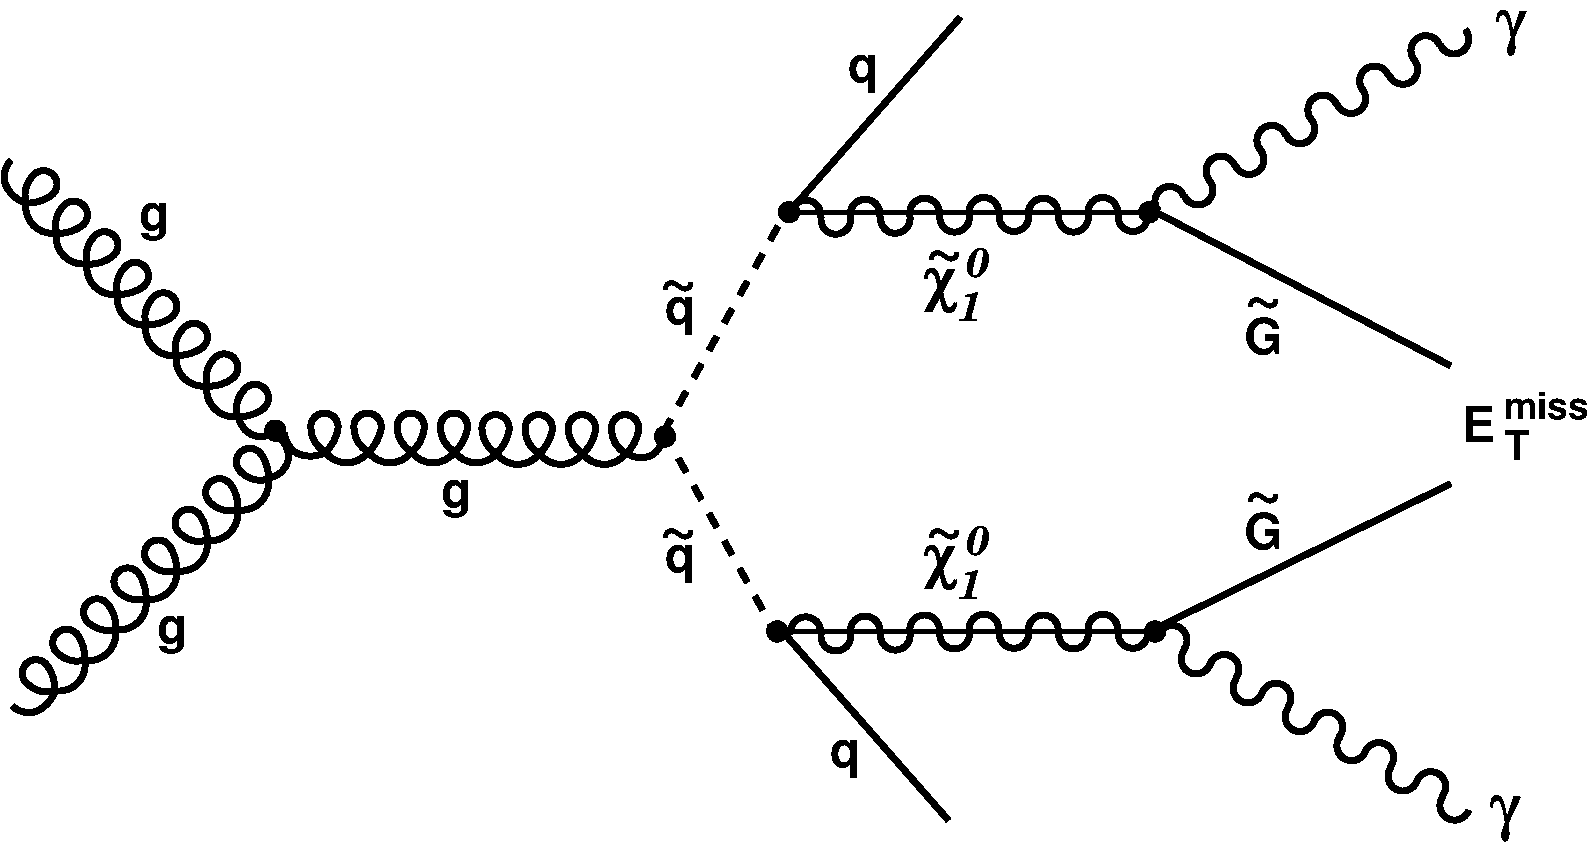
\includegraphics[width=0.50\linewidth]{THESISPLOTS/Diphoton_squark.pdf}
       
     \large{ \textcolor{red}{2 Photons}, \textcolor{green}{2 Jets}, \textcolor{blue}{Large MET} }   
   %  }
     \end{varblock}%
     \vspace{-0.3cm}
     \begin{varblock}[7cm]{Single Photon}
  %\fbox{
    \centering
       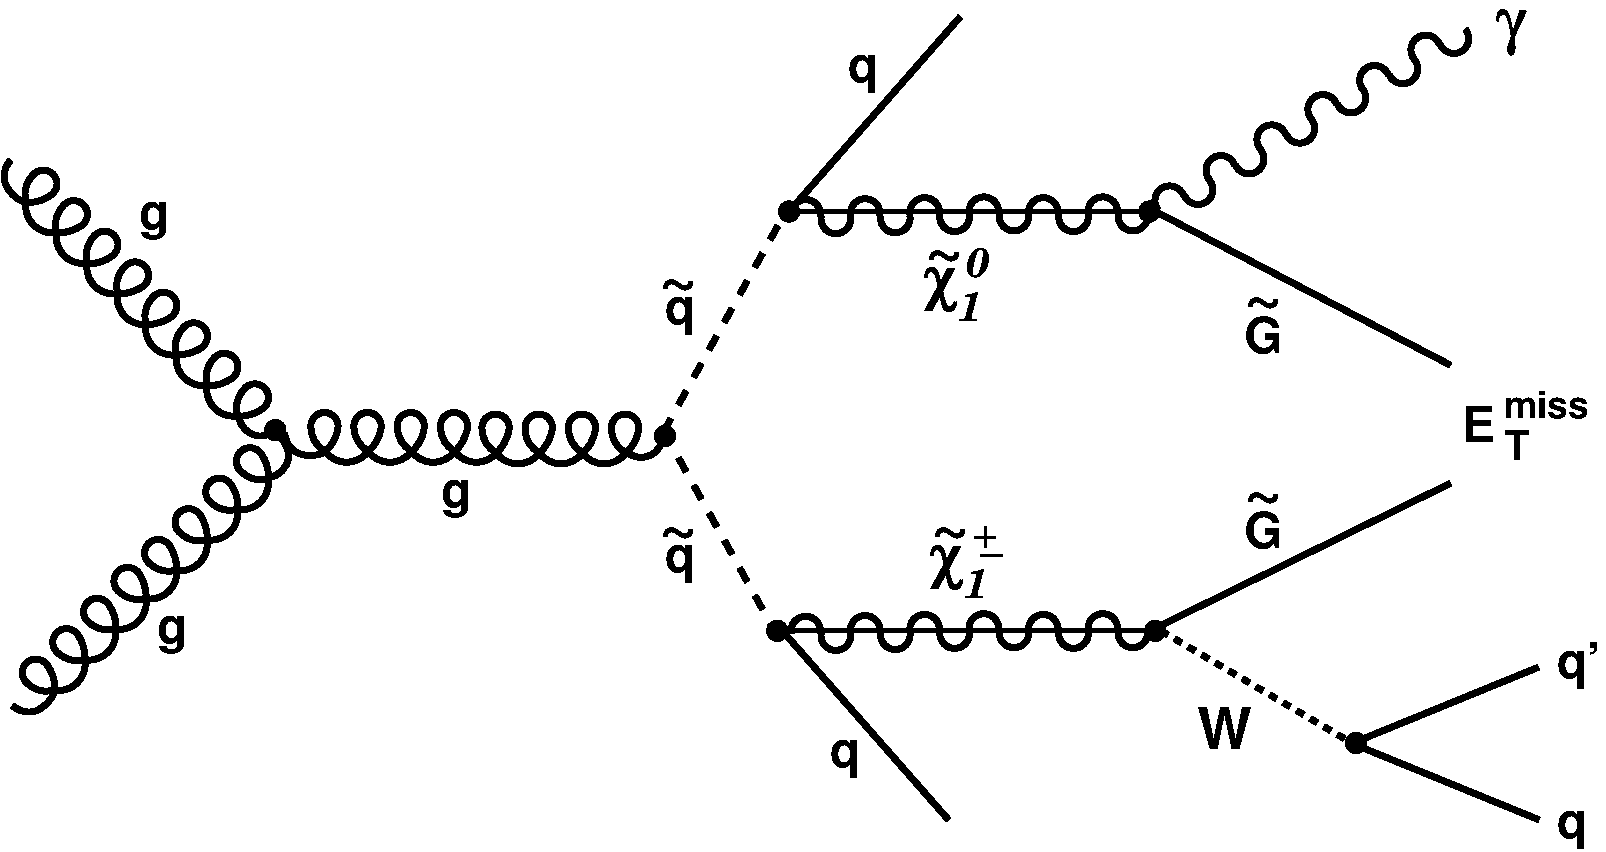
\includegraphics[width=0.50\linewidth]{THESISPLOTS/SinglePhoton_squark.pdf}
       \newline
       \large{ \textcolor{red}{1 Photon}, \textcolor{green}{Jets}, \textcolor{blue}{Large MET} }
  %     }
    \end{varblock}
   % \end{minipage}
 % \end{column}
 % \hspace{-4.5cm}
  % Column 2 begins
%  \begin{column}{0.9\textwidth}  
%    \begin{minipage}[t]{0.5\textwidth}
%     \centering
%      \includegraphics[height=7cm,width=1.1\linewidth]{THESISPLOTS/SUSY-XSEC.pdf}
      %\includegraphics[scale=0.4]{THESISPLOTS/SUSY-XSEC.pdf}
%    \end{minipage}
%    \end{column} 
% \end{columns}     
\end{frame}

% Tranverse Decay Distance
\begin{frame}
\frametitle{Tranverse Decay Distance}
\vspace{-0.70cm}
\begin{minipage}[t]{0.4\paperwidth}
   \begin{varblock}[6cm]{Distance Travelled}
     \begin{displaymath}
       \mathrm{L}_{T} = c\tau\cdot \left(\gamma \beta_{T} \right)  = c\tau \cdot \left(\frac{p_{T}}{m} \right)
      \end{displaymath}
    \end{varblock}
  
   \begin{varblock}[6cm]{Proper Decay Length}
    \begin{displaymath}
    c\tau_{\texttt{NLSP}} = C^{2}_{\texttt{grav}}\frac{1}{\kappa}\left(\frac{m_{\texttt{NLSP}}}{ GeV}\right)^{-5}\left(\frac{\sqrt{\texttt{F}}}{TeV}\right)^{4}
     \end{displaymath}
    \end{varblock}    
\end{minipage} 
  
\begin{minipage}[b]{0.65\paperwidth}
    \includegraphics[width=0.75\paperwidth]{THESISPLOTS/DECAY-RATES.pdf}
     \newline \texttt{\textcolor{blue}{J. Ruderman, D. Shih arXiv:1103.6083}}
\end{minipage} 
   
 % begin{minipage}[b]{0.5\textwidth}
  %\texttt{Y. Kats et al}: arXiv:1110.6444v2
 %\end{minipage}
\end{frame}


%DataSet and Trigger Section
\section{Dataset and Trigger}
\begin{frame}
\frametitle{\Huge Datasets}
%\hspace{-0.2cm}
\begin{minipage}[b]{0.7\paperwidth}
\begin{itemize}
 \item  \textcolor{UMN@Maroon}{\textbf{Data~($19.1 fb^{-1} $)}}
  %\begin{varblock}[7cm]{Data~($19.1 fb^{-1}$) and Signal MC}
   %\centering
   \tinyv{
   \begin{tabular}{l l p{1.2cm}|p{1.9cm}|}
    \hline
       \bfseries{Dataset Name} & \bfseries{Recorded Luminosity} $ [fb^{-1}]$ \\ %$[\fbinv]$ \\
       \hline
       \texttt{/Run2012B/SinglePhoton/EXODisplacedPhoton-PromptSkim-v3 } & 5.1 \\
       \texttt{/Run2012C/SinglePhoton/EXODisplacedPhoton-PromptSkim-v3 } & 6.9 \\
       \texttt{/Run2012D/SinglePhoton/EXODisplacedPhoton-PromptSkim-v3 } & 7.1 \\
       \hline\hline
       \texttt{/Run2012C/Cosmics/Run2012C-22Jan2013-v1/RECO } & 3130384(\texttt{events}) \\
       \texttt{/Run2012D/Cosmics/Run2012C-22Jan2013-v1/RECO } & 52430 (\texttt{events}) \\
       \hline\hline
       \texttt{/SingleElectron/Run2012A-22Jan2013-v1/AOD} & 5.2 \\
       \texttt{/DoubleElectron/Run2012C-22Jan2013-v1/AOD} & 4.8 \\ 
       \hline \hline     
   \end{tabular}
       }
   \end{itemize}
 \end{minipage}
   % \vspace{1cm}
   % \hspace{0.5cm}
    
 \begin{minipage}[b]{0.7\paperwidth}
 \begin{itemize}
    \item  \textcolor{UMN@Maroon}{\textbf{Signal MC [GMSB~(SPS8)]}}
    %\centering
    \tiny{
    
%     \begin{tabular}{l l l l}
%     %\hline
%       %\textbf{Signal MC [mGMSB~(SPS8)]}
%        \hline
%        \bfseries{$\Lambda$}~[TeV] & \bfseries{$c\tau$}~(mm) & \bfseries{$\sigma_{LO}$}~(pb) & \bfseries{Number of events}\\
%       \hline
%       100 & 250-12,000  & 0.368  & 60,000 \\
%       120 & 250-12,000  & 0.133  & 60,000 \\
%       140 & 250-12,000  & 0.0574 & 60,000 \\
%       160 & 250-12,000  & 0.0277 & 60,000 \\
%       180 & 250-12,000  & 0.0145 & 60,000 \\
%       \hline \hline
%       \end{tabular} 
%\renewcommand\arraystretch{1.2}
%\centering
\begin{tabular}{c c c c c c c}
\hline \hline
$\Lambda$~[TeV] & 100  &   120  &  140  &  160  &  180  &  300  \\
\hline
$M_{\tilde{\chi}^{0}_{1}}$~[$GeV/c^{2}$] & 140 &   169  &  198  &  227  &  256  &  430  \\
\hline
$c\tau$         &  215   &   325  &   130 &   245 &   185 &       \\
 (mm)     &  425   &   645  &   515 &   490 &   365 &   495 \\
                 &  1700  &  1290  &  1030 &   975 &   730 &       \\
                 &  3400  &  1935  &  2060 &  1945 &  1100 &   995 \\
                 &  5100  &  2955  &  2920 &  2930 &  2195 &  2960 \\
                 &  6000  &  3870  &  3985 &  3910 &  3950 &       \\
                 &  9300  &  5985  &  6000 &  5875 &  5980 &  6000 \\
                 &        &  9825  & 10450 &  9815 & 10450 & 10450 \\
\hline \hline
    \end{tabular}
    
}
        
    \end{itemize} 

\end{minipage} 
 
 \begin{minipage}[b]{0.7\paperwidth}
 \begin{itemize}
   \item \textcolor{UMN@Maroon}{ \textbf{$\gamma +$ Jets MC}}
     \mytiny{  
     \begin{tabular}{l l l}
        %\hline
         %
       \hline
        $\hat{p}_{T}$~[GeV\ /c] & $\sigma_{LO}$~(pb) & \bfseries{Number of events}\\
       \hline
       $50 - 80$ & 3322.3  & 1995062 \\
       $80 - 120$ &  558.3  & 1992627 \\
       $120 - 170$  &  108.0 & 2000043 \\
       $170 - 300$  &  30.1 & 2000069 \\
       $300 - 470$  &  2.1  & 2000130 \\
       $470 - 800$  & 0.212 & 1975231 \\
       \hline \hline
       \end{tabular}  
       }
    \end{itemize}
     
    \end{minipage}
% \end{varblock} 
 \end{frame}
 
 % HLT Trigger
 \begin{frame}
 \frametitle{\huge{HLT Trigger}}
  \begin{minipage}[b]{\linewidth}
  %\begin{varblock}[7.2cm]{HLT-Trigger Efficiency}
    \begin{itemize}
     \item \textbf{HLT\_DisplacedPhoton65\_CaloIdVL\_IsoL\_PFMET25}%~(\texttt{Main Trigger})
     \begin{itemize}
        \item  HLT\_Photon50\_CaloIdVL\_IsoL (\texttt{Study Trigger})
     \end{itemize}
   \end{itemize}  
  %\end{varblock}
  \end{minipage}
  
  
 \vspace{-0.2cm}
 \begin{minipage}[b]{0.7\paperwidth}
 %\begin{itemize}
 %\centering{
 % \textcolor{UMN@Maroon}{\textbf{HLT-Trigger Efficiency}} }
  %\vspace{-0.5cm}
\flushleft
    \begin{figure}[htbp]
 \mbox{
   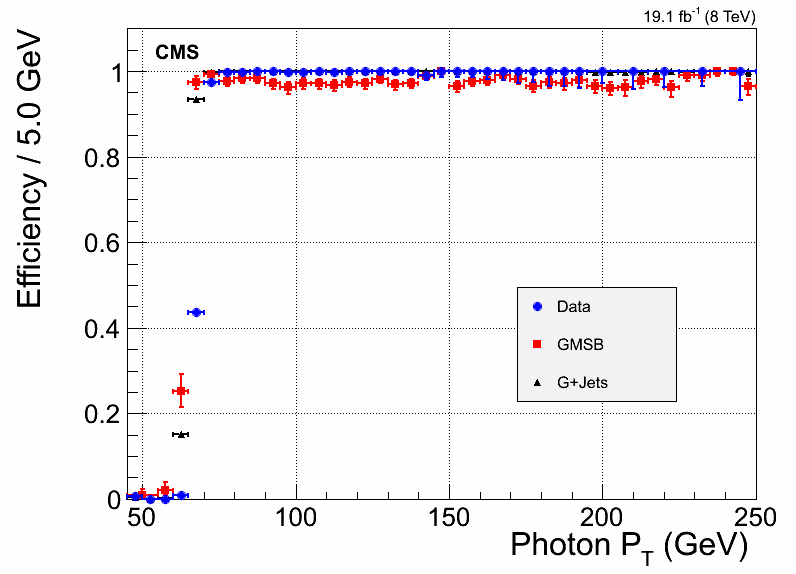
\includegraphics[height=4.0cm,width=0.55\textwidth]{THESISPLOTS/Photon_EffAsym.png}
   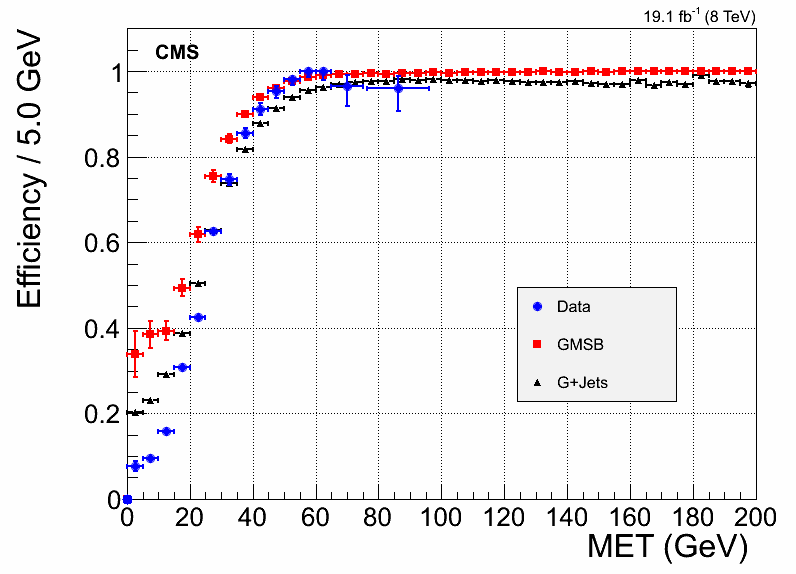
\includegraphics[height=4.0cm,width=0.55\textwidth]{THESISPLOTS/PFMET_EffAsym.png} }
  %  \vspace{-0.80cm}
 %\caption{\tiny{\alert{(LEFT)}: $c\tau=6000$~mm, \alert{(RIGHT)}: $c\tau=12000$~mm}}
   \end{figure}    
 % \end{itemize}
\end{minipage}  
\centering
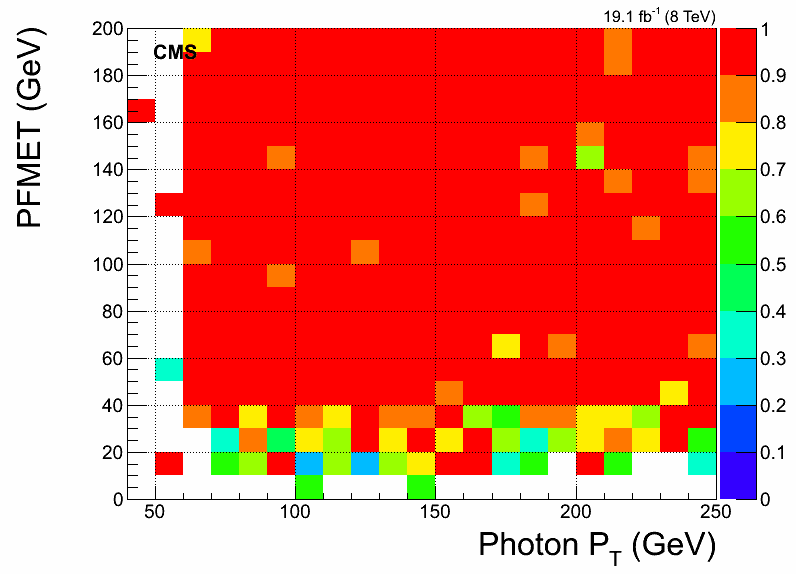
\includegraphics[height=3.5cm,width=0.70\textwidth]{THESISPLOTS/Eff2D.png} 
  
  
 % \end{itemize}
\end{frame}


% ECAL Timing
%\section{ECAL Timing}
\begin{frame}
\frametitle{\huge{ECAL Timing}}
 \begin{minipage}[b]{0.8\paperwidth}
  \begin{itemize}
   \item\textcolor{UMN@Maroon}{\textbf{Time Reconstruction}} 
      \begin{itemize}
        \item 10 digitized samples used.
        \item Fit and Weighted methods used to extract time.
      \end{itemize}   
   \item \textcolor{UMN@Maroon}{\textbf{Time Measurement}}
      %\begin{equation*}\label{eq:avetime}
 $$  T_{MAX} = \frac{{\displaystyle\sum_{i}} \frac{T_{MAX,i} }{\sigma_i^2} }{ {\displaystyle\sum_{i}} \frac{1}{\sigma_i^2} } $$
     %\end{equation}
  \end{itemize}   
\end{minipage}
 
 \begin{minipage}[b]{0.8\paperwidth}
   \begin{itemize}
    \item \textcolor{UMN@Maroon}{\textbf{Time Performance}}
    \begin{itemize}
     \item  Time resolution better than $200$~ps for $E > 30$ ~GeV
    \end{itemize}
     
   \end{itemize}
 \end{minipage}
 \mbox{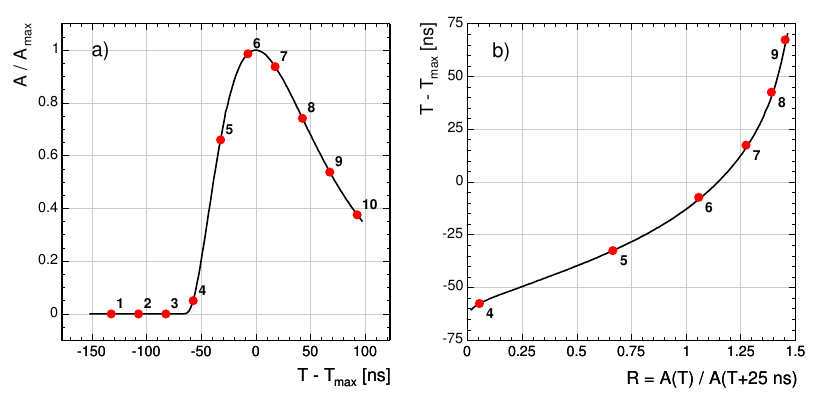
\includegraphics[height=3.0cm,width=0.50\textwidth]            {THESISPLOTS/AmplitudeVsTMax.png}
      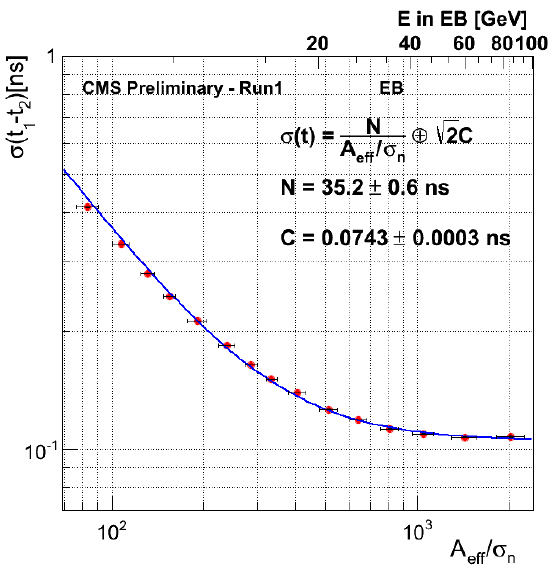
\includegraphics[height=3.0cm,width=0.50\textwidth]            {THESISPLOTS/NeigboMethodECALTimeRes.png}}
\end{frame}

%continuation of Timing
\begin{frame}
\frametitle{\huge{ECAL Timing(2)}}
  \begin{minipage}[b]{0.8\paperwidth}
   \begin{itemize}
    \item \textcolor{UMN@Maroon}{\textbf{Photon Timing}}
        \begin{itemize}
         \item $T_{\gamma} =$ Average Time of all Crystals.
         \item $T_{\gamma} =$ Seed (most energetic) Crystal Time.
        \end{itemize}
      
       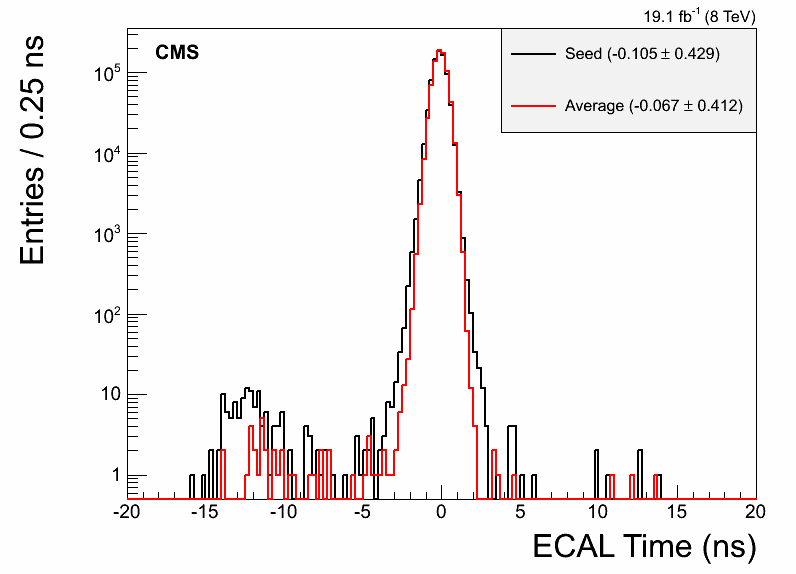
\includegraphics[height=5.0cm,width=0.70\textwidth]            {THESISPLOTS/AverageVsSeedTime_ECAL.png}   
  \end{itemize}
  \begin{itemize}
   \item  Similar behavior seen in Seed and Average Time.
   \item  We use seed time as Photon Measured Time in this analysis.
  \end{itemize}
  
 \end{minipage}
\end{frame}

\begin{frame}
\frametitle{\huge{ECAL Timing(3): MC Vs Data}}
  \begin{minipage}[b]{0.7\paperwidth}
    \begin{figure}[htbp]
    \mbox{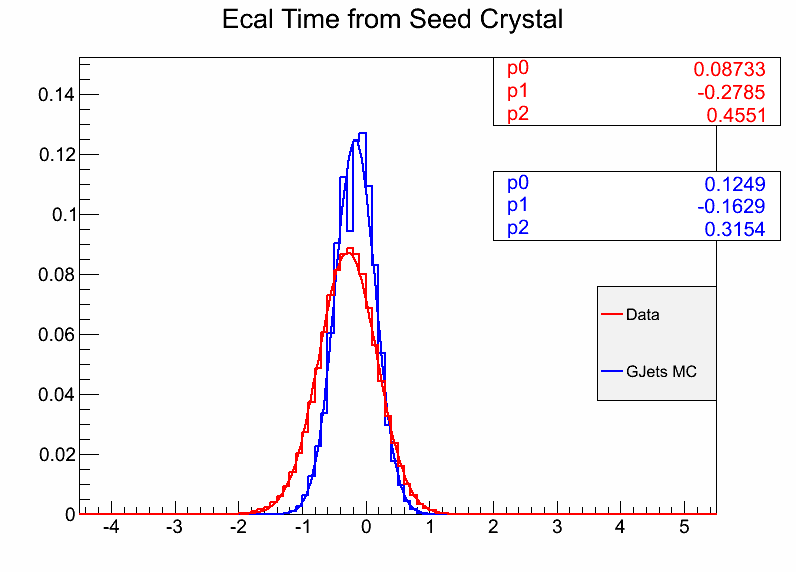
\includegraphics[height=5.0cm,width=0.61\textwidth]            {THESISPLOTS/SeedTime_data-mc.png}
          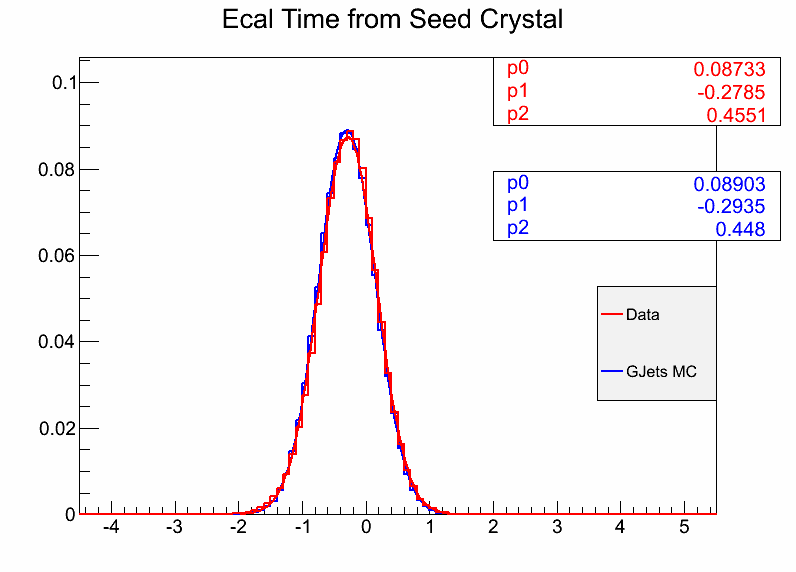
\includegraphics[height=5.0cm,width=0.61\textwidth]            {THESISPLOTS/SeedTime_data-mc_Calib.png}}
    \caption{\alert{(LEFT)}: Before \alert{(RIGHT)}: After}
   \end{figure} 
 \end{minipage}
 
 \begin{minipage}[b]{0.8\paperwidth}
  \begin{itemize}
     \item Timing corrections from data applied to $\gamma +$ Jets MC.
     \item $\gamma +$ Jets MC timing aligns better with data after corrections are applied.
  \end{itemize}
\end{minipage}
\end{frame}


%% Diagram of Why Long-Live Decay Kinematics
\begin{frame}
\frametitle{\huge {Long-Lived Decay}}
%\vspace{-1cm}
\begin{minipage}[t]{0.5\paperwidth}
  % \begin{varblock}[7cm]{Why Long-Lived?}
   \begin{itemize}
    \item \textcolor{UMN@Maroon}{\textbf{Source of Delayed Photon?}}
     \begin{itemize}
      \item Slow moving particle; $\beta << 1$,
      \item Non-nominal flight path,
      \item Stopped in subdetectors,
      %\item $\cdots$
     \end{itemize}
      
 \end{itemize}  
  % \end{varblock}
\end{minipage}

\begin{minipage}[t]{0.7\paperwidth}
\centering
  % 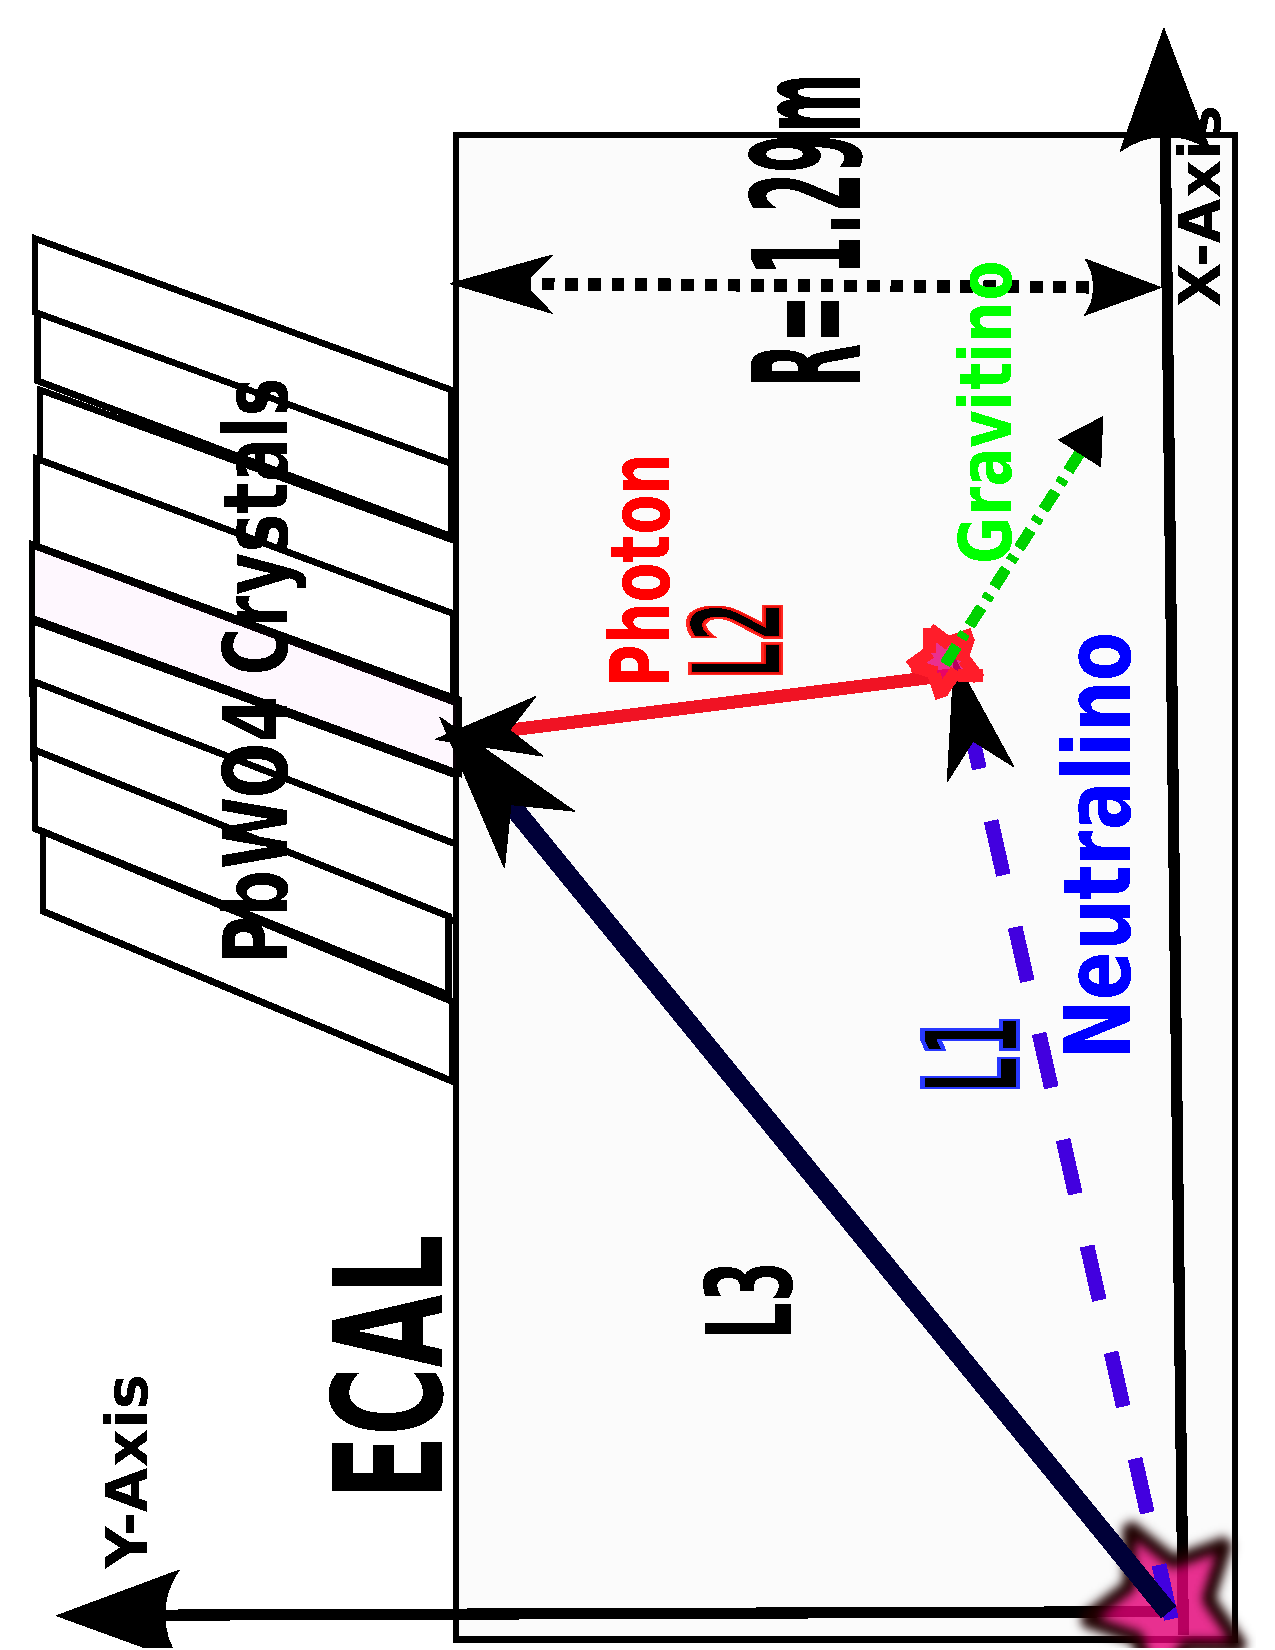
\includegraphics[height=9cm, width=0.45\paperwidth, angle=-90]{THESISPLOTS/Neutralino-Delayed-Photon-ECAL.pdf}
   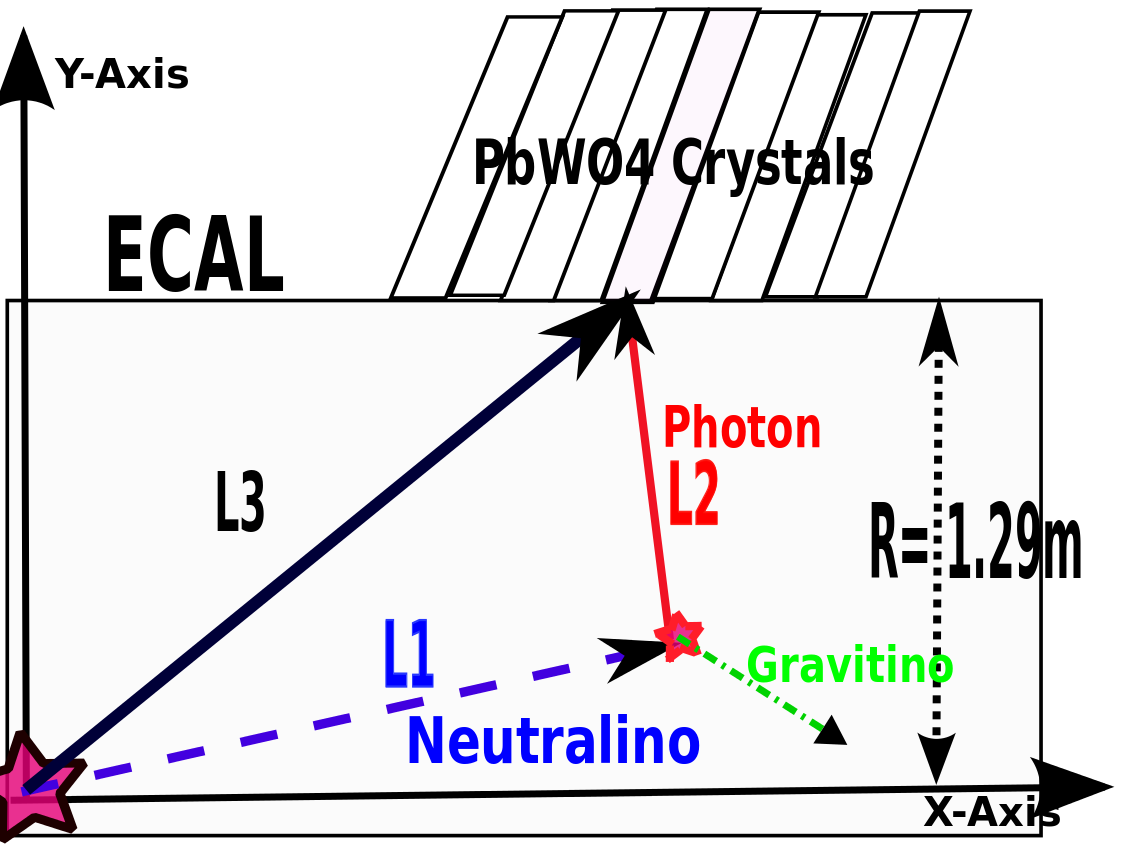
\includegraphics[height=6cm, width=0.8\paperwidth]{THESISPLOTS/DelayedPhoton-ECAL.png}
\end{minipage}
\end{frame}

%Long-Lived Or Offpoint
\begin{frame}
\frametitle{\huge{Slow Vs Off-Pointing Decay}}
  \begin{minipage}[t]{0.7\paperwidth}
    \begin{multicols}{2}
      \begin{varblock}[3.5cm]{Photon Arrival Time}
         
          $$\Delta t_{1} = (L1/c\beta) - (L1/c)$$
    
          $$\Delta t_{2} = (L1 + L2 - L3)/c $$   
           
      \end{varblock}
     \columnbreak
     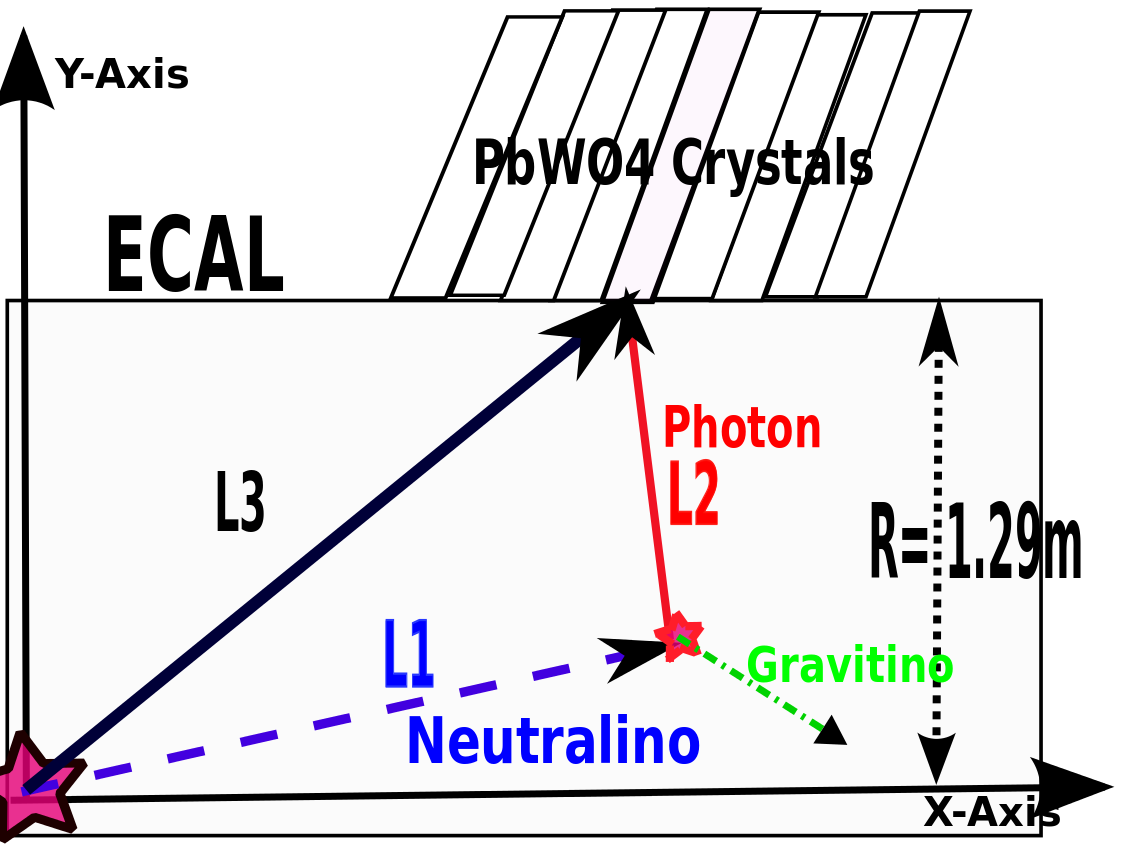
\includegraphics[height=3.30cm, width=0.4\paperwidth]{THESISPLOTS/DelayedPhoton-ECAL.png}
     
    \end{multicols} 
  \end{minipage}
  
  \begin{minipage}[t]{0.8\paperwidth}
    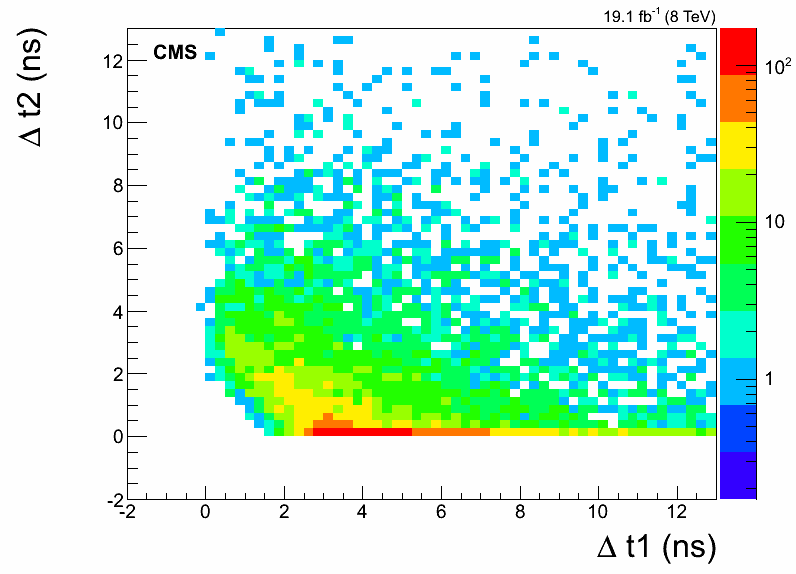
\includegraphics[height=3.8cm, width=0.7\paperwidth]{THESISPLOTS/dt1_dt2_late.png}
  \end{minipage}
  \vspace{-0.1cm}
  Delayed photons mostly from slow moving neutralino decays.

\end{frame}





% Event Selection
\section{Event Selection}
\begin{frame}
\frametitle{\Huge Event Selection}
%\subsection{Pre-Event Selection}
%\subsection{Event Cleaning}
%\subsection{Final Event Selection}
\begin{minipage}[b]{0.45\linewidth}
%\begin{center}
%\begin{table}[ht]
\centering
\small{
\begin{tabular}[2cm]{l l}
\multicolumn{2}{c}{\bfseries{Object Selection Criteria}} \\
  \hline 
  \bfseries{Variable} & \bfseries{Selection Cuts} \\
   \hline 
 % \texttt{primary vertex number of tracks(vnof)}& $>= 4$ \\
 % \texttt{primary vertex transverse distance to beam}~($d0$) & $ < 2$~cm from CMS center \\
%  \texttt{primary vertex longitudinal distance to beam}~($|z|$) & $ < 24$~cm from CMS center \\
  \texttt{Photon} $p_{T}(\gamma^{1(2)})$  & $ > 80(45)$~GeV \\
  %\texttt{Sub-Leading photon must have} $p_{T}(\gamma^{2})$  & $ > 45$~ GeV \\
 $|\eta_{\gamma}|$,(\texttt{EB only}),  &$ < 3.0$($ < 1.5$) \\
 \texttt{Semi-minor axis}($S_{Minor}$)  &$0.12 \leq S_{Minor} \leq 0.38$ \\
 \texttt{H/E}  & $ < 0.05$ \\
 \texttt{Track Vito},$\Delta R(\gamma, track)$  & $ > 0.6 $ \\
 \texttt{HCAL,ECAL, Track, Isolation}  & $ < 4.0 $,$ < 4.5 $,$ < 0.2 $ \\
 \texttt{Cone Size(Iso $\gamma$)} $\Delta R(\gamma, SC)$ & $< 0.4$ \\
 \texttt{Spike Swiss-Cross} & $1-E_{4}/E_{1})< 0.98$ \\ 
 %\texttt{Spike Swiss-Cross} & $1-E_{6}/E_{2} $,($1-E_{4}/E_{1})< 0.98$ \\ 
 % \hline 
%\end{tabular}
%\label{tab:PhotonSel}
%\end{table}
%\end{center}
%%\end{minipage}

%%\begin{minipage}[b]{0.55\linewidth}
%%\begin{center}
%\begin{table}[ht]
%%\centering
%%\begin{tabular}{ll}
%%\multicolumn{2}{c}{\bfseries{PF Jet Selection Criteria}} \\
  \hline 
  \hline
%%  \bfseries{Variable} & \bfseries{Selection Cuts} \\
%%   \hline 
 \texttt{Jets must satisfy} & \texttt{JetID Requirements} \\
 \texttt{Leading Jet} $p_{T}$ & $ > 35$~GeV \\
 \texttt{Number Of Constituents} & $ > 1$ \\
%% \texttt{Charge EM energy fraction~(CEF)}& $ < 0.99$ \\
%% \texttt{Neutral Hadron energy fraction~(NHF)}& $ < 0.99$ \\
%% \texttt{Neutral EM energy fraction~(NEF)}& $ < 0.99$ \\
% \texttt{If} $|\eta|$ \texttt{of jet is} $ >2.4$, \texttt{Charge Hadron energy fraction~(CHF) } & $ > 0$ \\
% \texttt{If} $|\eta|$ \texttt{of jet is} $ >2.4$, \texttt{Charge multiplicity~(NCH) } & $ > 0$ \\
 $\Delta R(\gamma, jet) = \sqrt{(\phi_{\gamma}-\phi_{jet})^{2} + (\eta_{\gamma}-\eta_{jet})^{2}}$ & $ > 0.3$ \\
\hline \hline
 $E^{\mbox{miss}}_{T}$&  $> 25$~GeV \\
 \hline
\end{tabular}
%\label{tab:JetSel}
%\end{table}
%\end{center}
}
\end{minipage}


%\centering
%\mbox{
%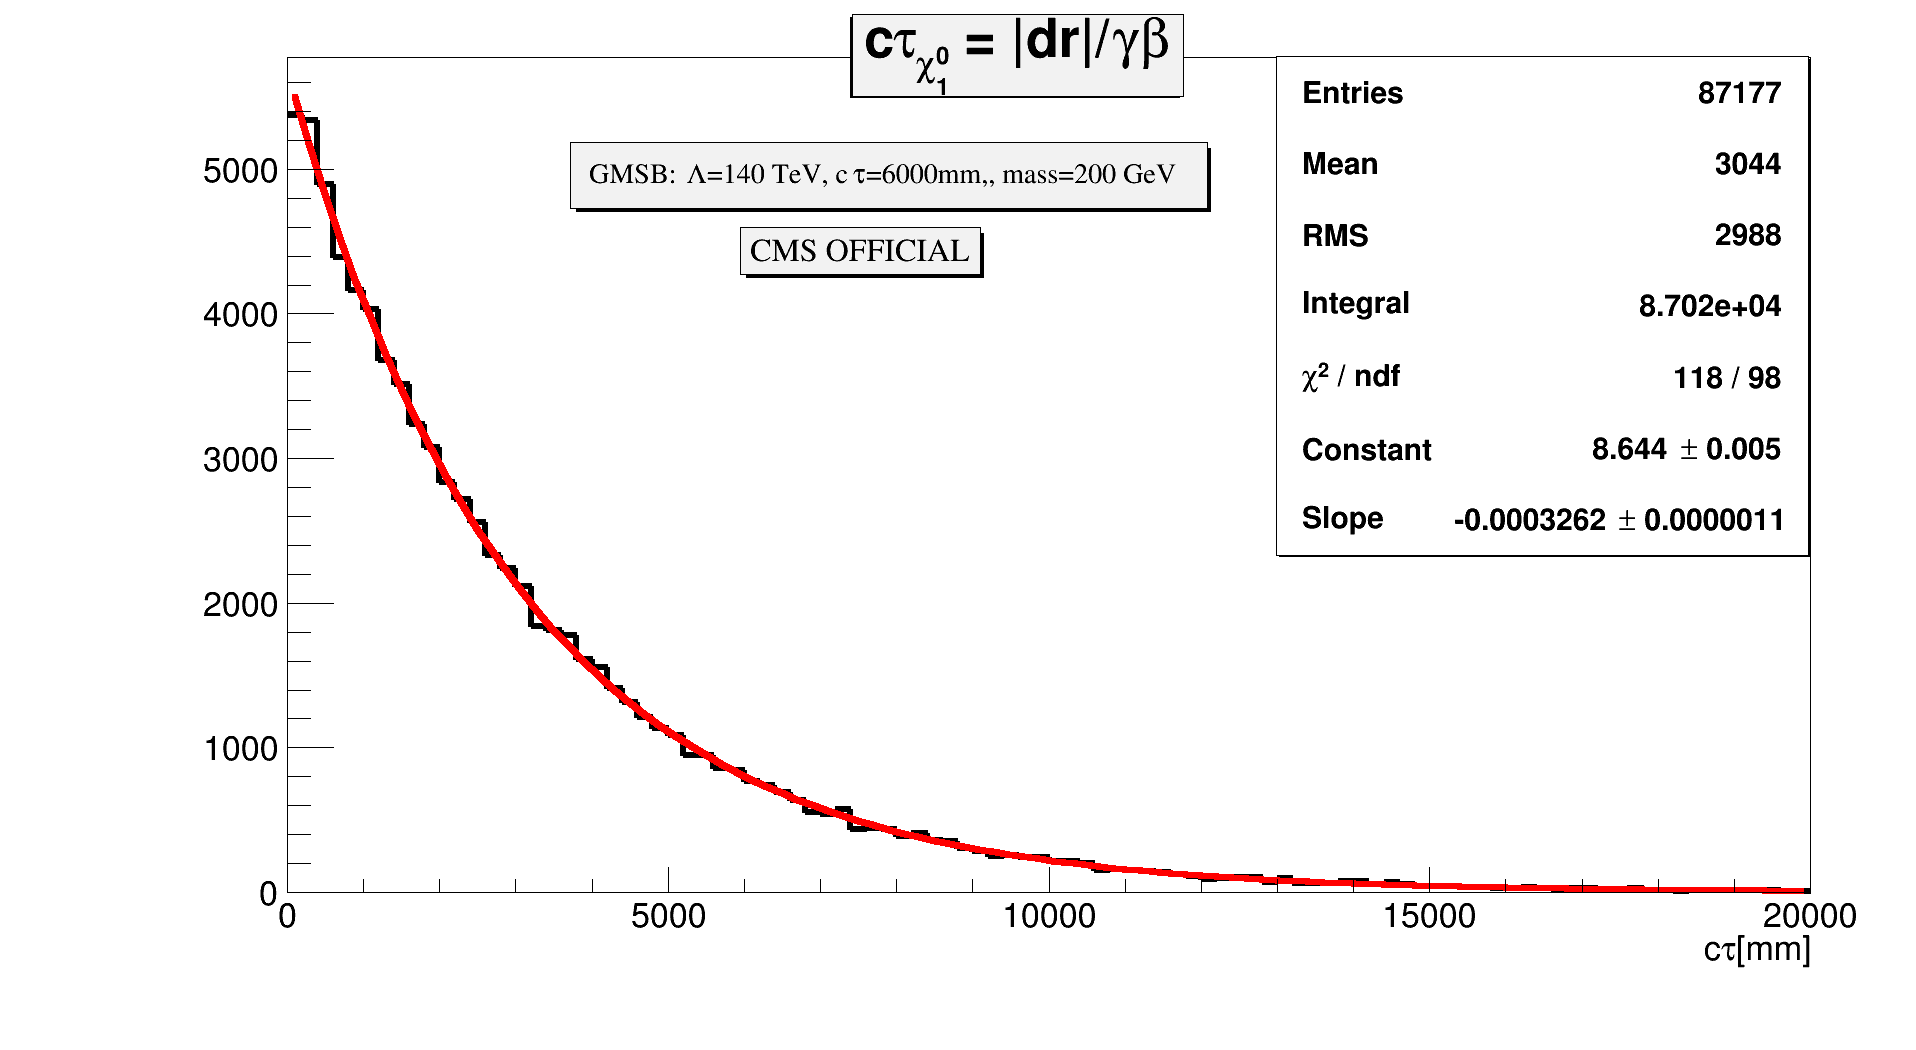
\includegraphics[height=6cm,width=\textwidth]{Dist_TravDL.png}}
%\vspace{-1cm}
%\caption{1/Slope = 3065.60 mm }
%\label{fig:Neutralino Distance}
%\end{minipage}
%\hspace{0.1cm}
%\begin{minipage}[b]{0.45\linewidth}
%\centering
%\mbox{
%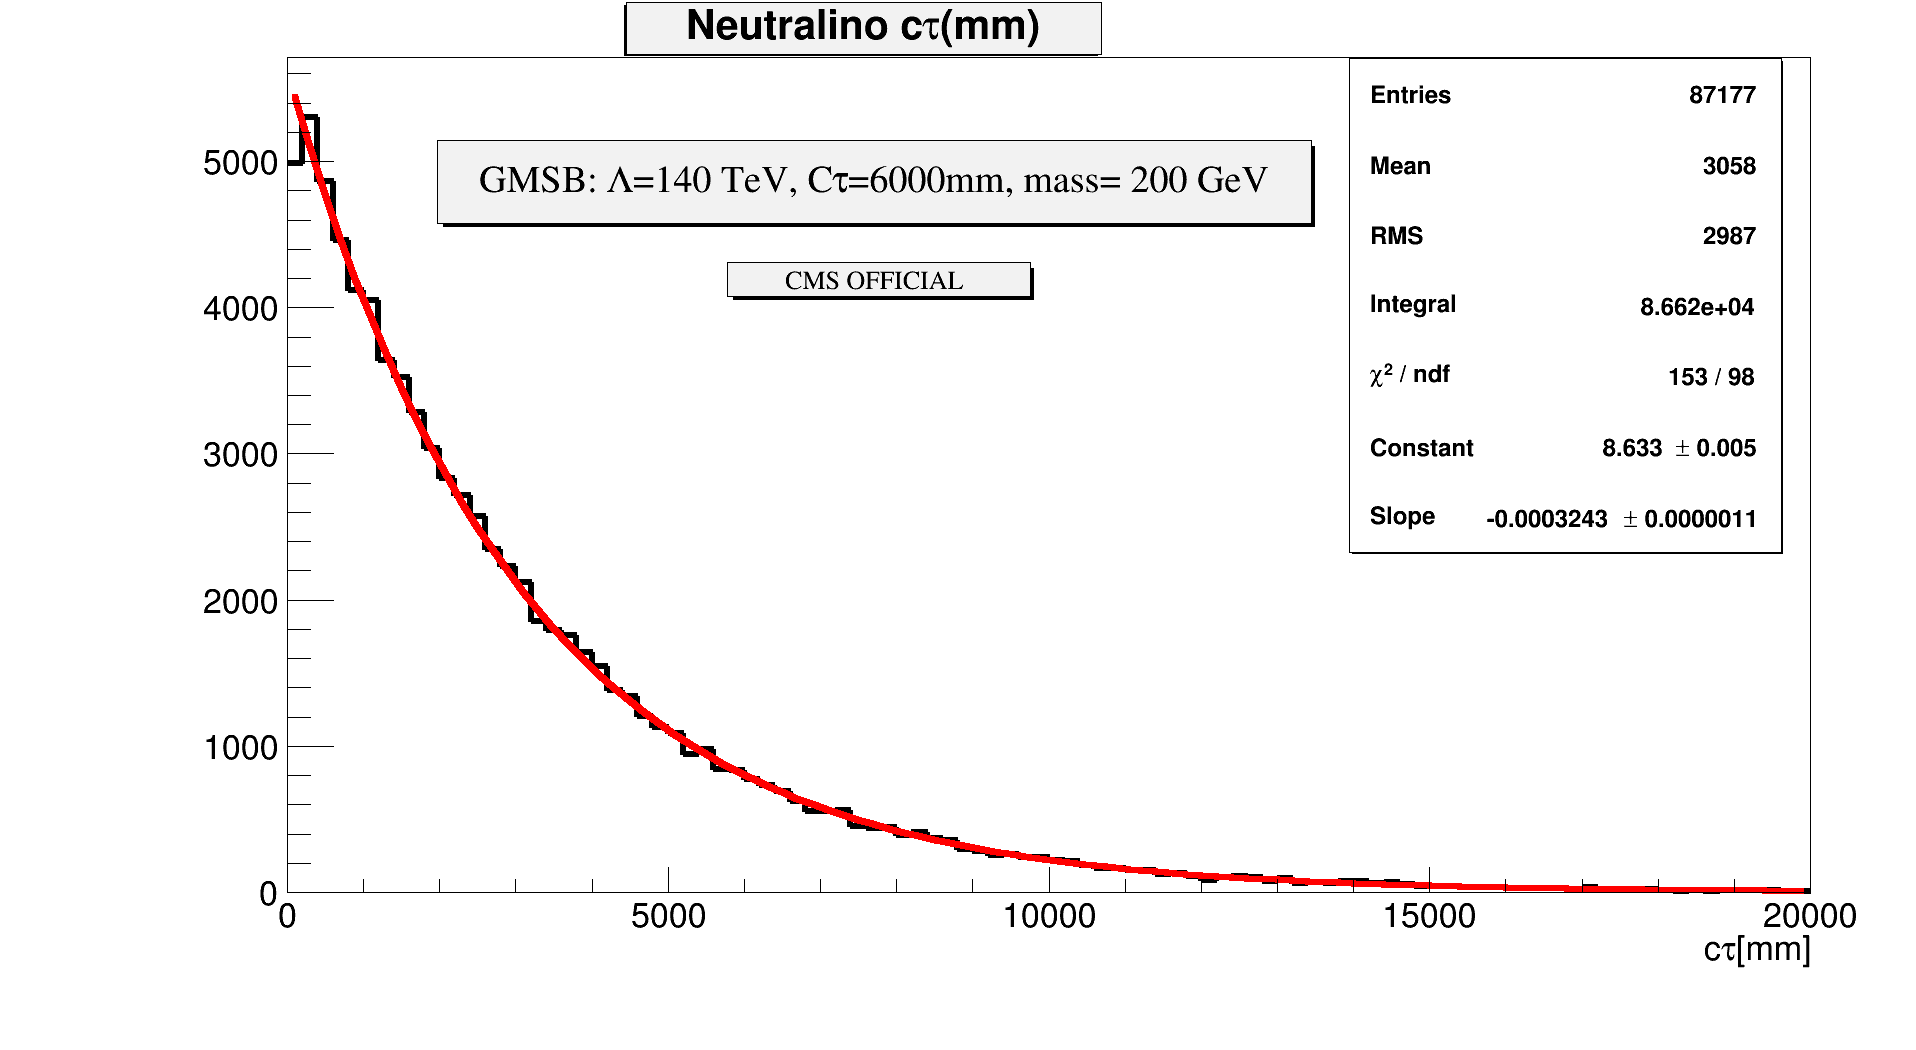
\includegraphics[height=6cm, width=\textwidth]{MC_TimeDL.png}}
%\vspace{-1cm}
%\caption{1/Slope = 3083.56 mm }
%\label{fig:From_MC}
%\end{minipage}
%\end{figure}
%\vspace{-1cm}
%\alert{\textbf{Sample is $c\tau= 6000$ mm but we measure $c\tau \approx 3000$ mm}}
\end{frame}

%% Decay Kinematics Distribution
\begin{frame}
\frametitle{Kinematics Distribution}
\begin{figure}[ht]
\begin{minipage}[b]{0.45\linewidth}
\centering
\mbox{
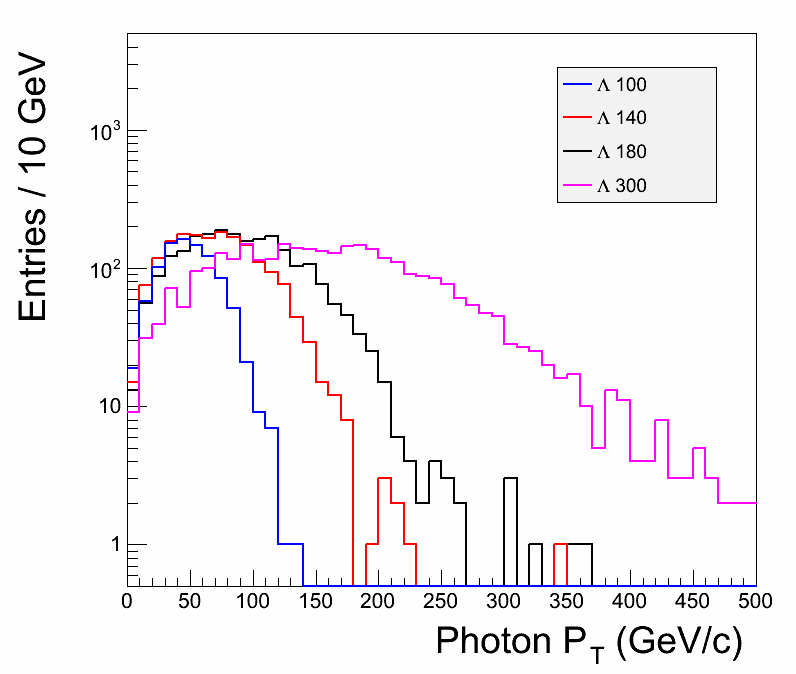
\includegraphics[height=6cm,width=\textwidth]{THESISPLOTS/GMSB_PhotPt.png}}
\vspace{-1cm}
\caption{Photon $p_{T}$}
%\label{fig:ctaulimit}
\end{minipage}
\hspace{0.1cm}
\begin{minipage}[b]{0.45\linewidth}
\centering
\mbox{
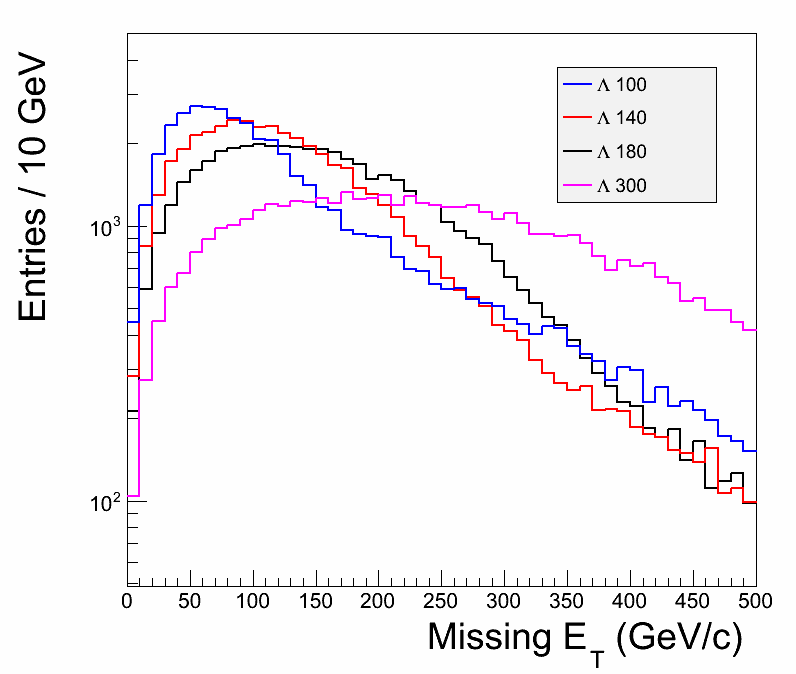
\includegraphics[height=6cm, width=\textwidth]{THESISPLOTS/GMSB_MET.png}}
\vspace{-1cm}
\caption{$E^{\mbox{miss}}_{T}$}
%\label{fig:masslimit}
\end{minipage}
\end{figure}
\begin{itemize}
 \item Different $\Lambda$ values with the same $c\tau$(10~m). Photon $p_{T}$ is harder with higher values of $\Lambda$.
\end{itemize}

\end{frame}

% Signal Efficiency & Acceptance
\begin{frame}
 \frametitle{Signal Efficiency and Acceptance}
\begin{figure}[ht]
\begin{minipage}[b]{0.45\linewidth}
\centering
\mbox{
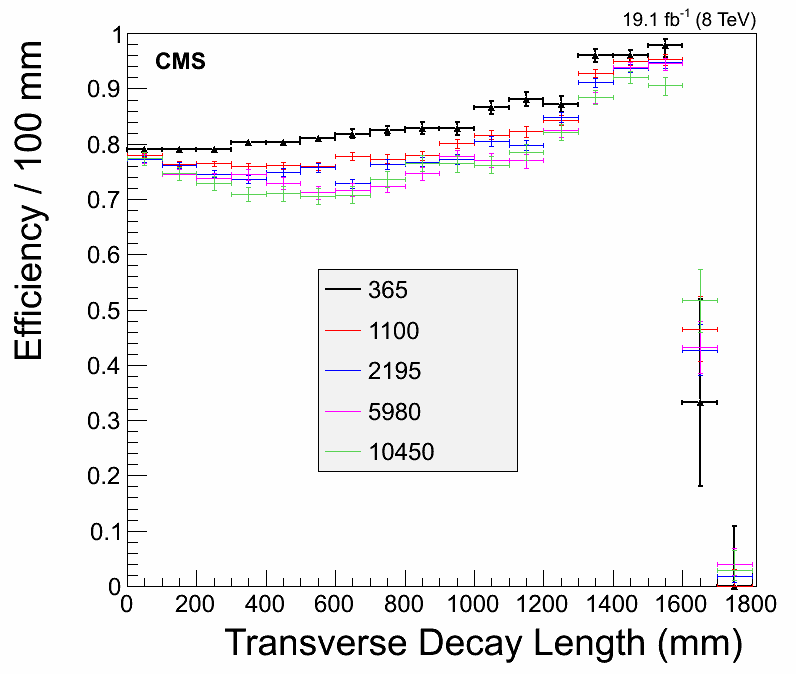
\includegraphics[height=6cm,width=\textwidth]{THESISPLOTS/Eff_ctbgT.png}}
\vspace{-1cm}
\caption{Efficiency}
%\label{fig:ctaulimit}
\end{minipage}
\hspace{0.1cm}
\begin{minipage}[b]{0.45\linewidth}
\centering
\mbox{
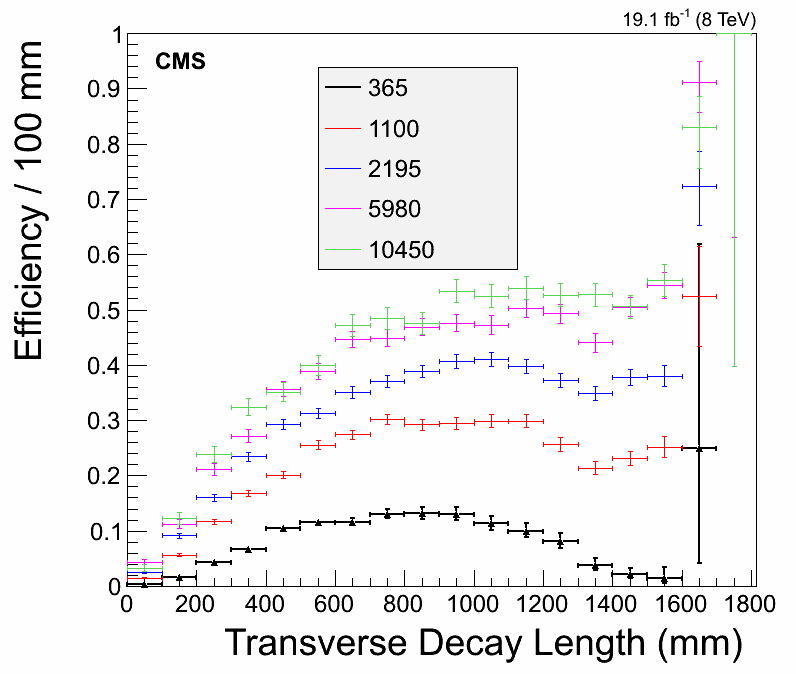
\includegraphics[height=6cm, width=\textwidth]{THESISPLOTS/Accp_ctbgT.png}}
\vspace{-1cm}
\caption{Acceptance}
%\label{fig:masslimit}
\end{minipage}
\end{figure}
 Sharp drop in efficiency immediately beyond ECAL radius for slow moving neutralino decay as source of delayed photon.

\end{frame}


\begin{frame}
 \frametitle{Signal Efficiency and Acceptance(II)}
\begin{figure}[ht]
\begin{minipage}[b]{0.45\linewidth}
\centering
\mbox{
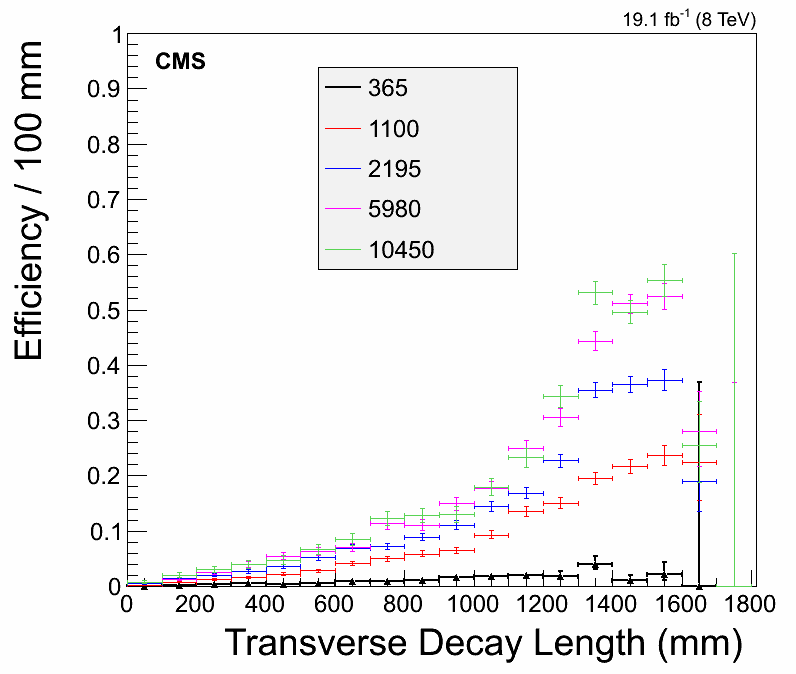
\includegraphics[height=6cm,width=\textwidth]{THESISPLOTS/Accp_ctbgT1.png}}
\vspace{-1cm}
\caption{Slow Moving}
%\label{fig:ctaulimit}
\end{minipage}
\hspace{0.1cm}
\begin{minipage}[b]{0.45\linewidth}
\centering
\mbox{
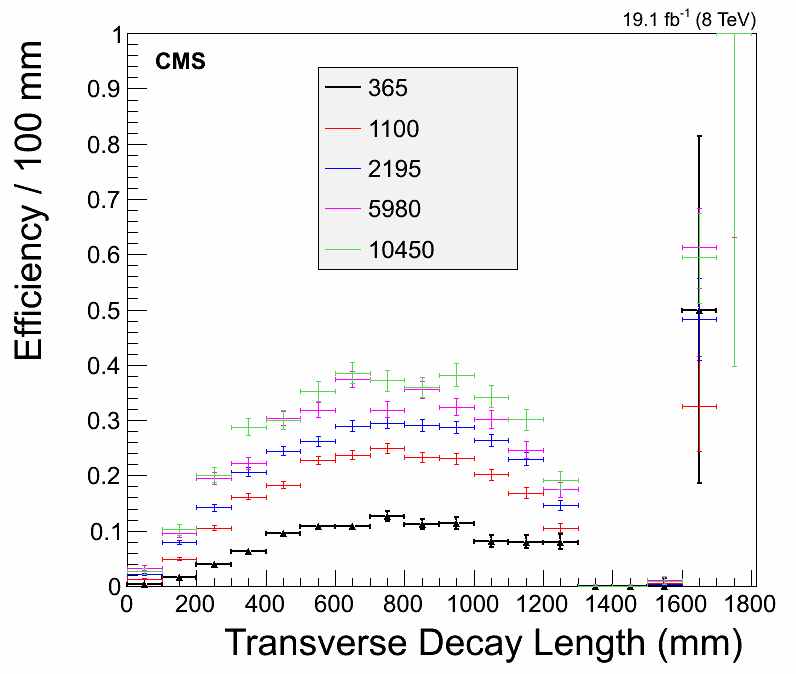
\includegraphics[height=6cm, width=\textwidth]{THESISPLOTS/Accp_ctbgT2.png}}
\vspace{-1cm}
\caption{Off-Pointing}
%\label{fig:masslimit}
\end{minipage}
\end{figure} 
 Acceptance peaks at transverse decay length 800~mm with delayed photons from off-pointing neutralino decays.
\end{frame}

\begin{frame}
\frametitle{Signal Efficiency and Acceptance(III)}
  \begin{figure}[ht]
   \begin{minipage}[b]{0.7\linewidth}
    \mbox{
  \centering
  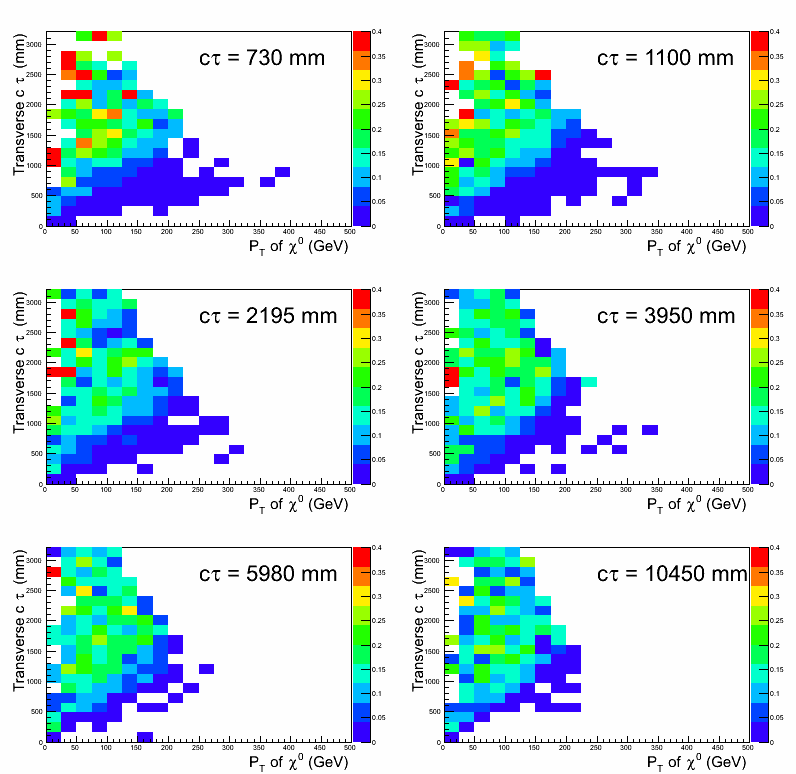
\includegraphics[height=7.5cm, width=0.65\paperwidth]{THESISPLOTS/Eff180_xPt_ct.png} }
    \vspace{-0.5cm}
    \caption{2 Dim Efficiency}
  \end{minipage}
 \end{figure}
\end{frame}



\section{Background Estimation}
%%%  Tagging and Efficiency
\begin{frame}
\frametitle{\Huge Sources Of Background}
  \begin{minipage}[t]{0.8\linewidth}
   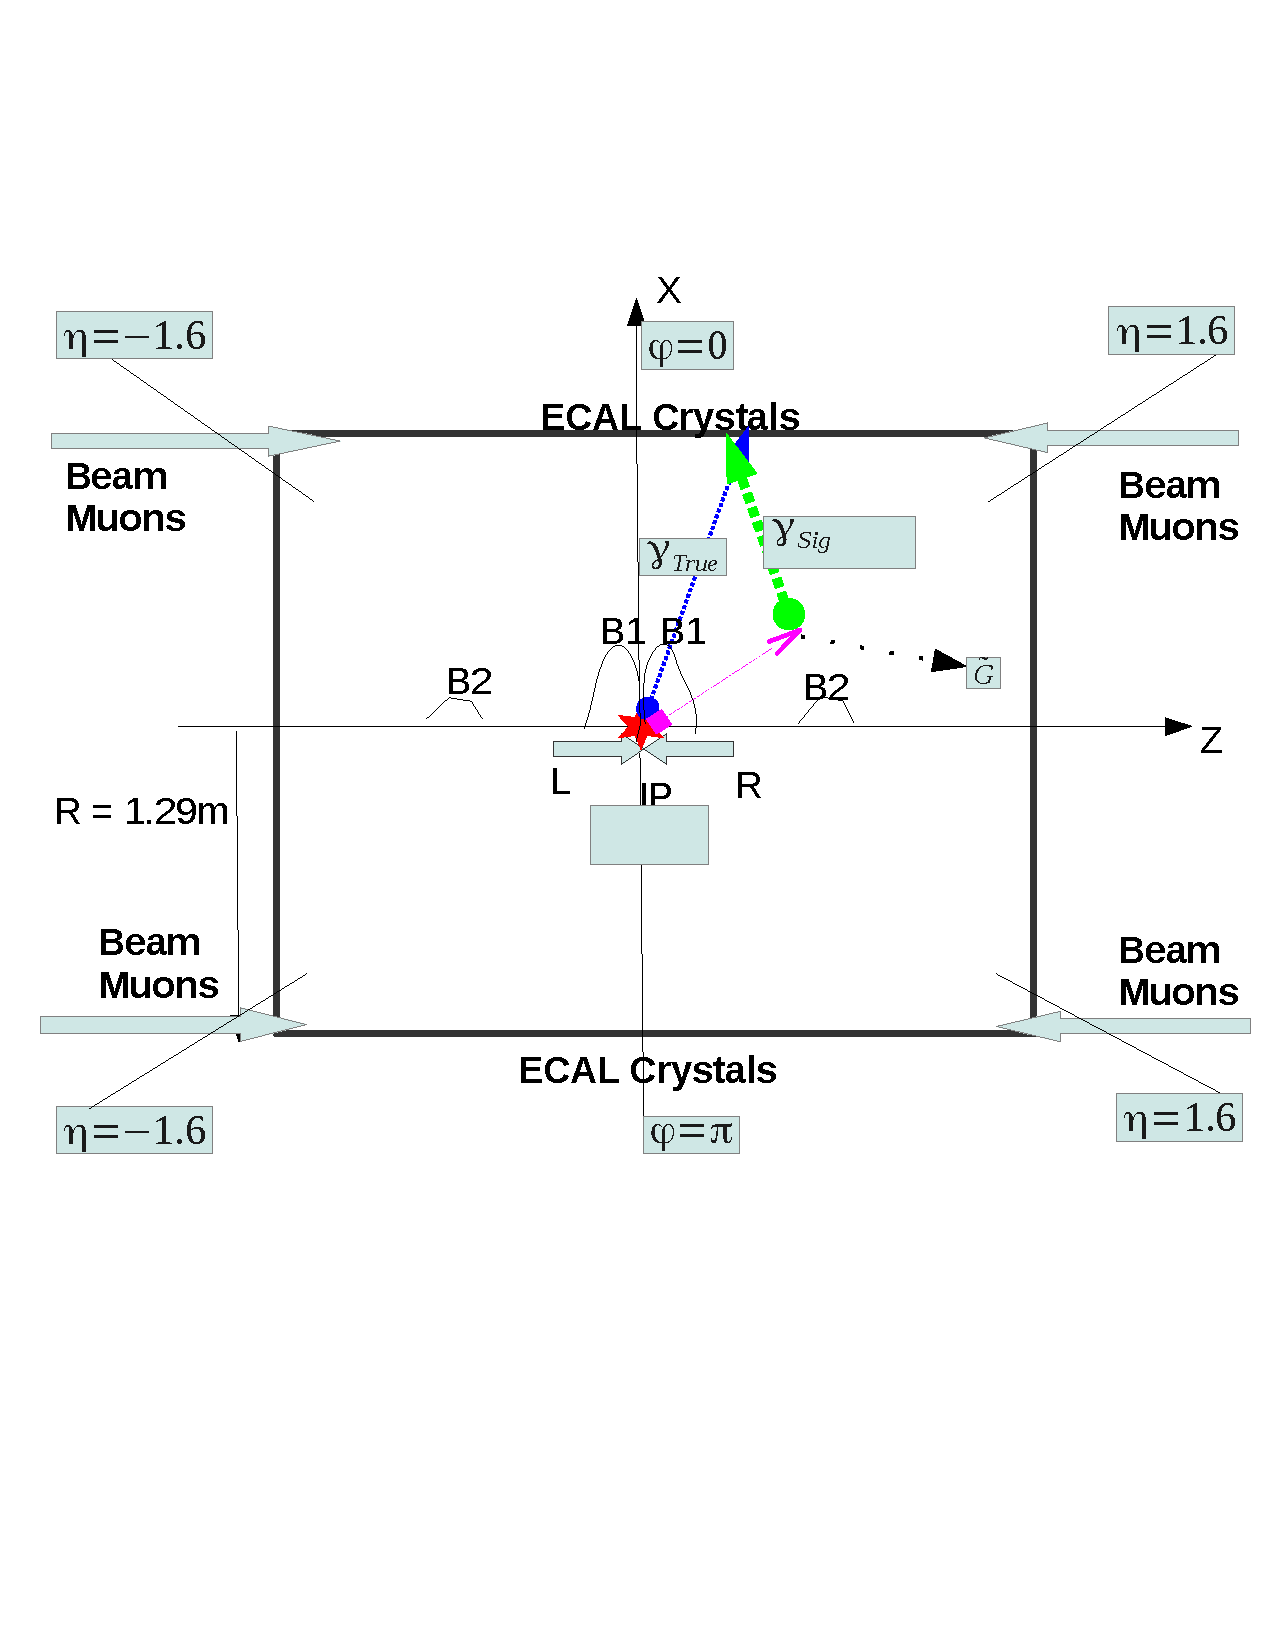
\includegraphics[width=\textwidth]{THESISPLOTS/Background_Delayed_Photon.pdf}
  \end{minipage}
% \begin{minipage}[t]{0.8\linewidth}
%  A combination of collision and non-collision events makes up delayed photon background sources.
% \end{minipage}
\end{frame}


\begin{frame}
\frametitle{\Huge Background Estimation}
 %\begin{figure}[ht]
  \begin{minipage}[t]{\linewidth}
   Main sources of background to delayed photons are:   
   \begin{itemize}
    \item Photons of events produced from Non-collision,
    \item Photons of events produced from collision with mis-measured ECAL time.
   \end{itemize}
  \end{minipage}
  
  \begin{minipage}[t]{\linewidth}
  %\begin{figure}[ht]
    %\centering
    \mbox{
 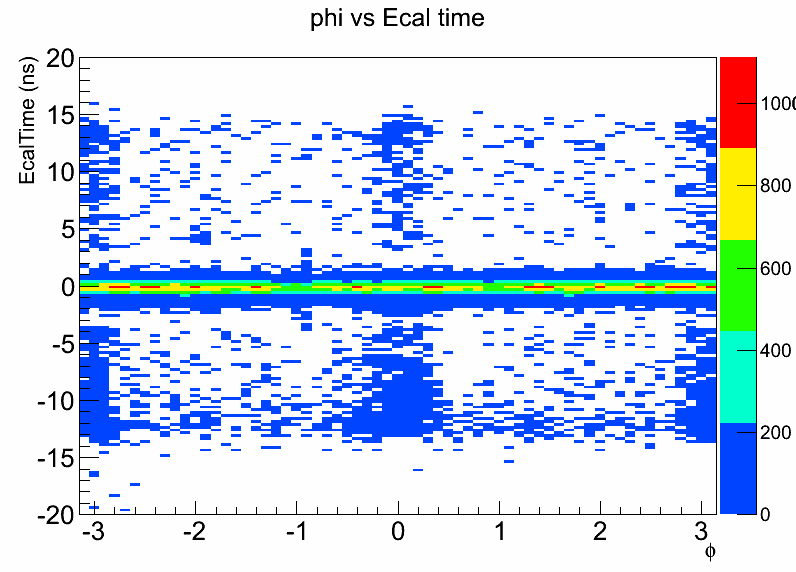
\includegraphics[width=0.40\paperwidth]{THESISPLOTS/h_Phi_Time.png}
 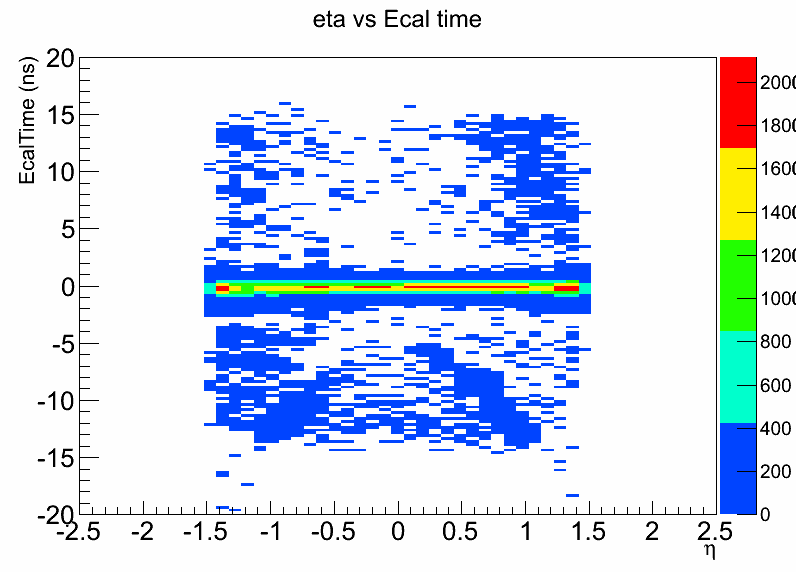
\includegraphics[width=0.40\paperwidth]{THESISPLOTS/h_Eta_Time.png} }
    %\vspace{-1cm}
    %\caption{Background}
   \end{minipage}
\begin{minipage}[b]{\linewidth}
Features around $\phi = 0, \pm \pi$ and $\eta$-dependence shows that background sources originate from both collision and non-collision events.
\end{minipage} 
 %\end{figure}
\end{frame}

\begin{frame}
\frametitle{In-Time Vs Out-Of-Time Events}
We estimate these background by defining two Control samples.
\begin{flushleft}
 \begin{description}
   \item[In-time] events Control Sample~(IT-CS)
   \item[Out-of-time] events Control Sample (OT-CS)
 \end{description} 
 \end{flushleft}
\begin{tcolorbox}[colback=blue!5,colframe=UMN@Maroon!40!black,title=Control Sample (In-time Events)]
%\lipsum[2]
\textbf{IT-CS}: $> 2$ Jets Events with photon ECAL time, $t \in [-1, 1]$~ns.
\end{tcolorbox}

\begin{tcolorbox}[colback=blue!5,colframe=UMN@Maroon!40!black,title=Control Sample (Out-Of-time Events)]
%\lipsum[2]
\textbf{OT-CS}: $0$ Jet Events with photon ECAL time, $ t < -3$~ns or $t > 2$~ns.
\end{tcolorbox}
 
 \begin{minipage}[t]{0.8\linewidth}
 Events from above CSs provide a unique approach to estimate possible background contribution in signal.
 \end{minipage}
\end{frame}




%% Halo Photon
\begin{frame}
\frametitle{Halo Photon (HP)}
 \begin{tcolorbox}[colback=blue!5,colframe=UMN@Maroon!40!black,title=Beam Halo Muons]
\begin{itemize}
 \item Proton beam interacting with gas/air particles in the beam pipe,
 \item Proton beam colliding with the collimators upstream prior to entering the CMS detector.
\end{itemize}
will produce energetic muons traveling parallel with main proton beam and showering in the Calorimeters.
\end{tcolorbox}
 \begin{minipage}[t]{0.8\linewidth}
  \mbox{
   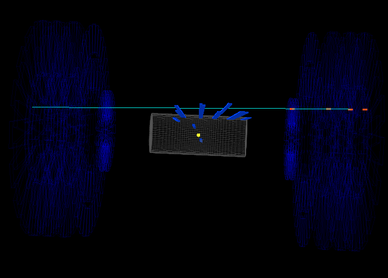
\includegraphics[height=3.7cm,width=0.40\paperwidth]{THESISPLOTS/Beam_Halo-CandidateEvent24186728-Run122314.png}\quad
   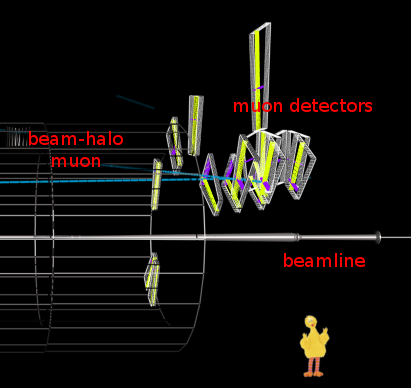
\includegraphics[height=3.7cm,width=0.40\paperwidth]{THESISPLOTS/beam_halo_csc.png}
  }   
 \end{minipage}
\end{frame}

%halo Photons
\begin{frame}
\frametitle{Halo Photon (II)}
   \begin{minipage}[t]{\linewidth}
    Using Halo kinematics, We can tag and estimate halo photons produced from halo muons showering in ECAL as follows:
    \begin{columns}
      \column{0.5\textwidth}
       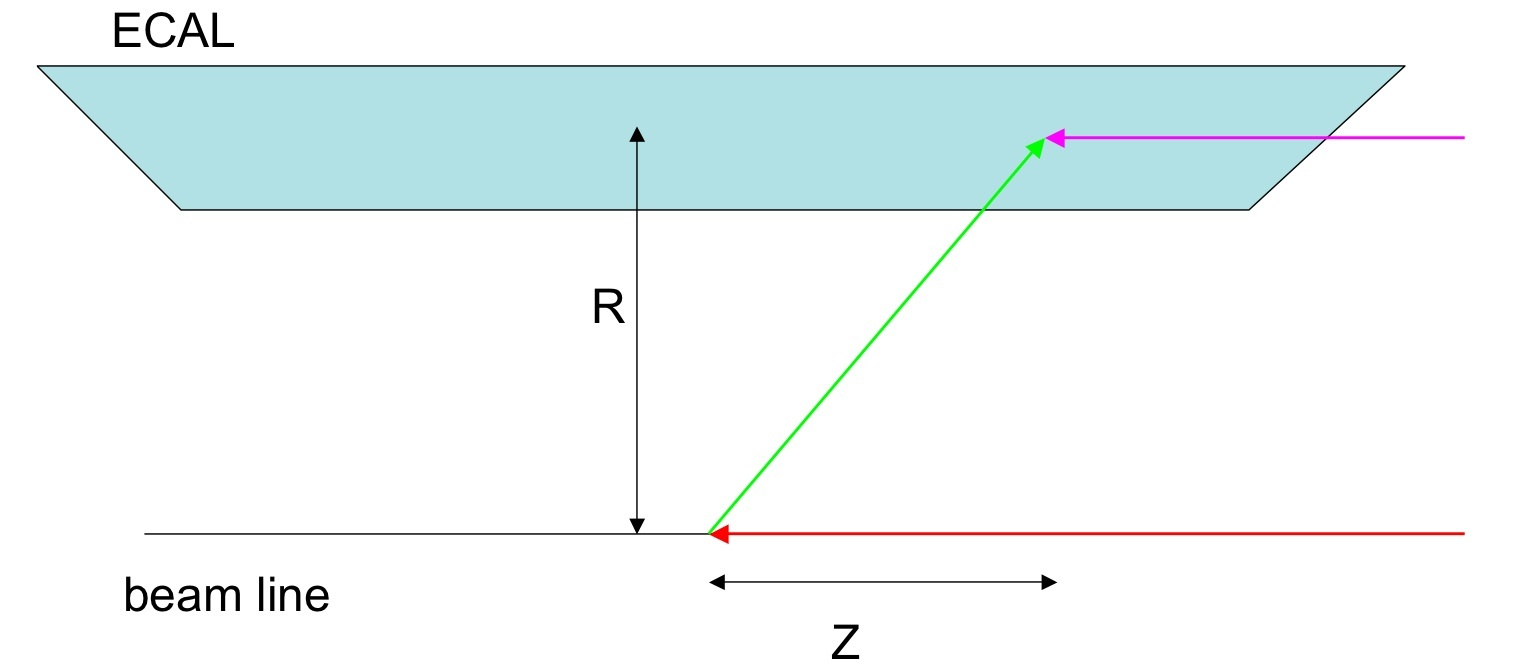
\includegraphics[height=3.7cm,width=0.40\paperwidth]{THESISPLOTS/Halo-Schematic-Diagram.jpg}
      \column{0.5\textwidth}
      \begin{varblock}[3.7cm]{Halo Expected Time}
          \begin{eqnarray*}
              t_{0} &=& \frac{\rho}{c} = \frac{R}{\sin\theta}.\frac{1}{c}\\
              t_{halo} &=& \frac{Z}{c} = \frac{R}{\tan\theta}.\frac{1}{c} \\
          \Delta t^{H}_{ECAL} &=& t_{halo}- t_{0} = \frac{Z}{c} - \frac{\rho}{c} \\
                    \Delta t^{exp}_{H}      &=&-\frac{R}{2c}\exp^{-\eta}
         \end{eqnarray*}
        \end{varblock}     
      \end{columns}
   \end{minipage}
   
   \begin{minipage}[t]{0.8\linewidth}
   \mbox{
     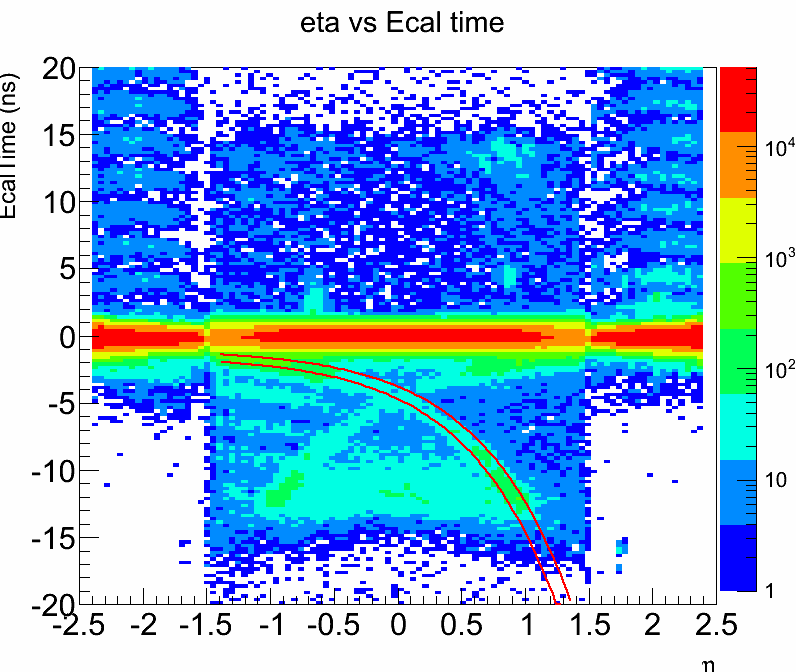
\includegraphics[height=3.4cm,width=0.40\paperwidth]{THESISPLOTS/HaloFunction.png} \quad
     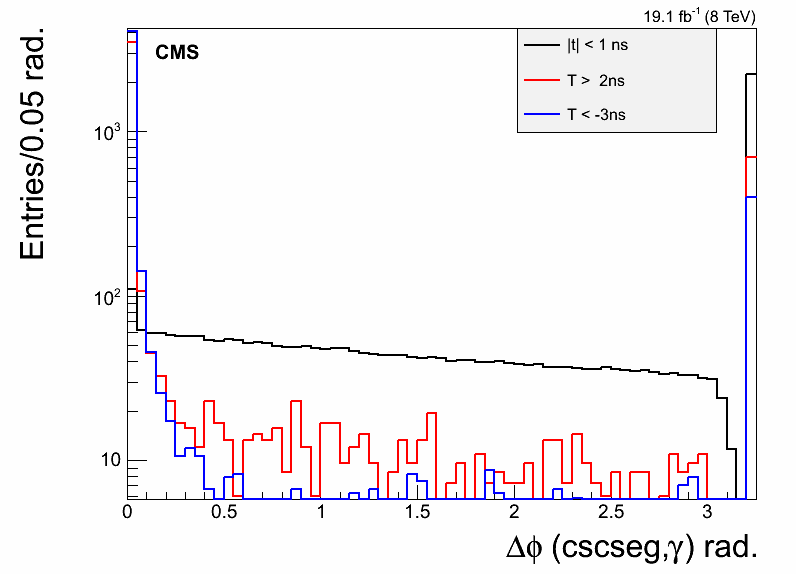
\includegraphics[height=3.4cm,width=0.40\paperwidth]{THESISPLOTS/cs_side_cscdPhi.png}
    }
   \end{minipage}
\end{frame}
%% Halo Photon Efficiency & Mis-tagging rate
\begin{frame}
\frametitle{HP Tagging Efficiency/mis-Tag Rate}

\end{frame}



%% Cosmic Muons
\begin{frame}
\frametitle{Cosmic Muons}
 \begin{minipage}[t]{0.8\linewidth}

 \end{minipage}
\end{frame}

%% Anomalous Events
\begin{frame}
\frametitle{Anomalous ECAL Spike}
 \begin{minipage}[t]{0.8\linewidth}

 \end{minipage}
\end{frame}

\begin{frame}
\frametitle{ABCD Technique: Non-Collision Background}
\end{frame}

\begin{frame}
\frametitle{ABCD Technique: Collision Background}
\end{frame}

\begin{frame}
\frametitle{ABCD Technique: Total Background Estimation}
  Equations and Results.
 \begin{minipage}[t]{0.8\linewidth}

 \end{minipage}
 
 \textbf{Closure Test}: Events with $1-jet$.
 \begin{minipage}[t]{0.8\linewidth}

 \end{minipage}
\end{frame}

\begin{frame}
\frametitle{Background Estimation Cross-Check}
Using $Z \rightarrow ee$ events.
\end{frame}





%%Systematic Uncertainties
\section{Systematics}
\begin{frame}
\frametitle{\Huge Systematics}
 \begin{minipage}[t]{0.8\linewidth}
  Background estimation is Data driven.
  Thus, most of a systematics come from signal,including:
  \begin{varblock}[7cm]{Experimental Systematics}
   \begin{itemize}
    \item Definition of Absolute or Zero time,
    \item ECAL time Resolution,    
    \item Unclustered Energy,
    \item Jet energy scale,
    \item Jets energy resolution,
    \item Photon energy scale,
    \item Luminosity. We use standard CMS luminosity uncertainty.
   \end{itemize}
  \end{varblock}  
  \begin{varblock}[7cm]{Theoretical Systematics}
   \begin{itemize}   
   \item Choice of PDF.
   \item Re-normalization group equations.
   \end{itemize}
  \end{varblock} 
\end{minipage}
\end{frame}

\begin{frame}
\frametitle{\Huge Systematics(II)}
\begin{minipage}[t]{0.8\textwidth}
\centering
\begin{tabular}{l l}
\multicolumn{2}{c}{\bfseries{Systematic Uncertainties}} \\
  \hline 
   \bfseries{Source} & \bfseries{Uncertainty(\%)} \\
   \hline
   \texttt{Absolute time(Zero time)}& $10\sim 6$  \\
   \texttt{Unclustered Energy}&  $10 \sim 4 $  \\
   \texttt{Photon Energy Scale}& $ 4 \sim 2$  \\
   \texttt{ECAL Time Resolution}& $ 5 \sim 2 $   \\
   \texttt{Jet Energy Scale}& $9 \sim 3$   \\
   \texttt{Jet Energy Resolution}& $ 9 \sim 2 $  \\
   \hline
   \texttt{Luminosity} & 2.6    \\
   \texttt{Choice of PDF} & $ < 1$ \\
  \hline \hline
 \end{tabular} 
 \end{minipage}
 
 \begin{minipage}[b]{0.8\textwidth}
 \begin{itemize}
  \item Systematics is obtained by studying the effects of varying by a few amount of a particular source of systematic on the total number of objects passing object selection cuts.
   \end{itemize}
 \end{minipage}
\end{frame}

%Results
\section{Results}
\begin{frame}
\frametitle{Results}
\begin{minipage}[t]{0.8\textwidth}
\centering
\begin{tabular}{l l l}
\multicolumn{3}{c}{\bfseries{Events Passing Final Selection}} \\
  \hline
   \bfseries{Sample} &\bfseries{Lifetime($c\tau$)[mm]} &\bfseries{Number Of Events} \\
   \hline
   \texttt{GMSB $\Lambda=180$ TeV}& $10500$ & \\
   \texttt{GMSB $\Lambda=180$ TeV}& $ 6000$ &  \\
   \texttt{GMSB $\Lambda=180$ TeV}& $ 4000$&  \\
   \texttt{GMSB $\Lambda=180$ TeV}& $ 3000 $&   \\
   \texttt{GMSB $\Lambda=180$ TeV}& $ 2000$&   \\
   \texttt{GMSB $\Lambda=180$ TeV}& $ 1000$&  \\
   \texttt{GMSB $\Lambda=180$ TeV}& $ 500$&  \\
   \hline
   \texttt{Data} & 1.00 &    \\
   \texttt{Background Total} & $0.014$ & \\
  \hline \hline
 \end{tabular} 
 \end{minipage}

\end{frame}



\begin{frame}
\frametitle{\Huge CLs Upper Limits}
\begin{figure}[ht]
\begin{minipage}[b]{0.45\linewidth}
\centering
\mbox{
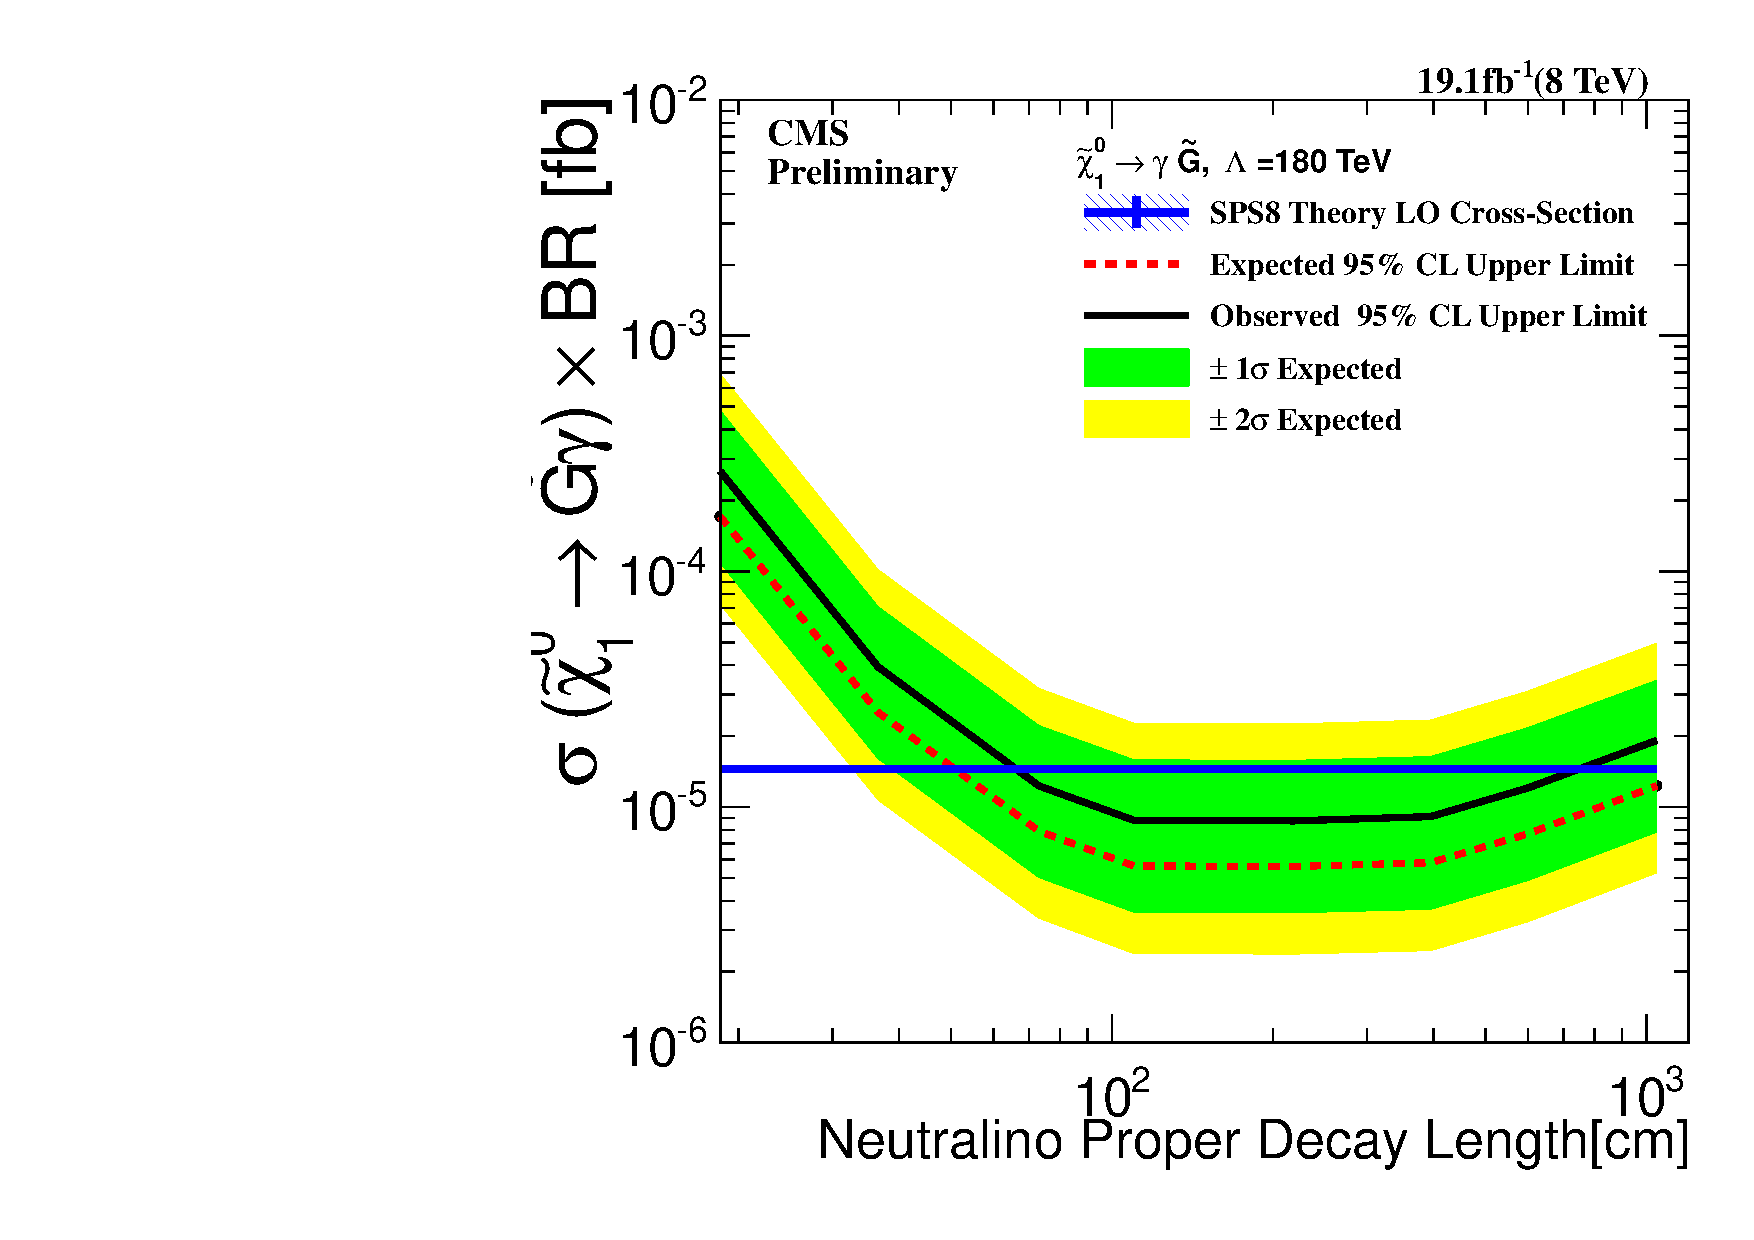
\includegraphics[height=6cm,width=\textwidth]{THESISPLOTS/180TeV_Neutralino_CrossSecTimesBR_Uplimit.pdf}}
\vspace{-1cm}
\caption{$c\tau$ Limits }
\label{fig:ctaulimit}
\end{minipage}
\hspace{0.1cm}
\begin{minipage}[b]{0.45\linewidth}
\centering
\mbox{
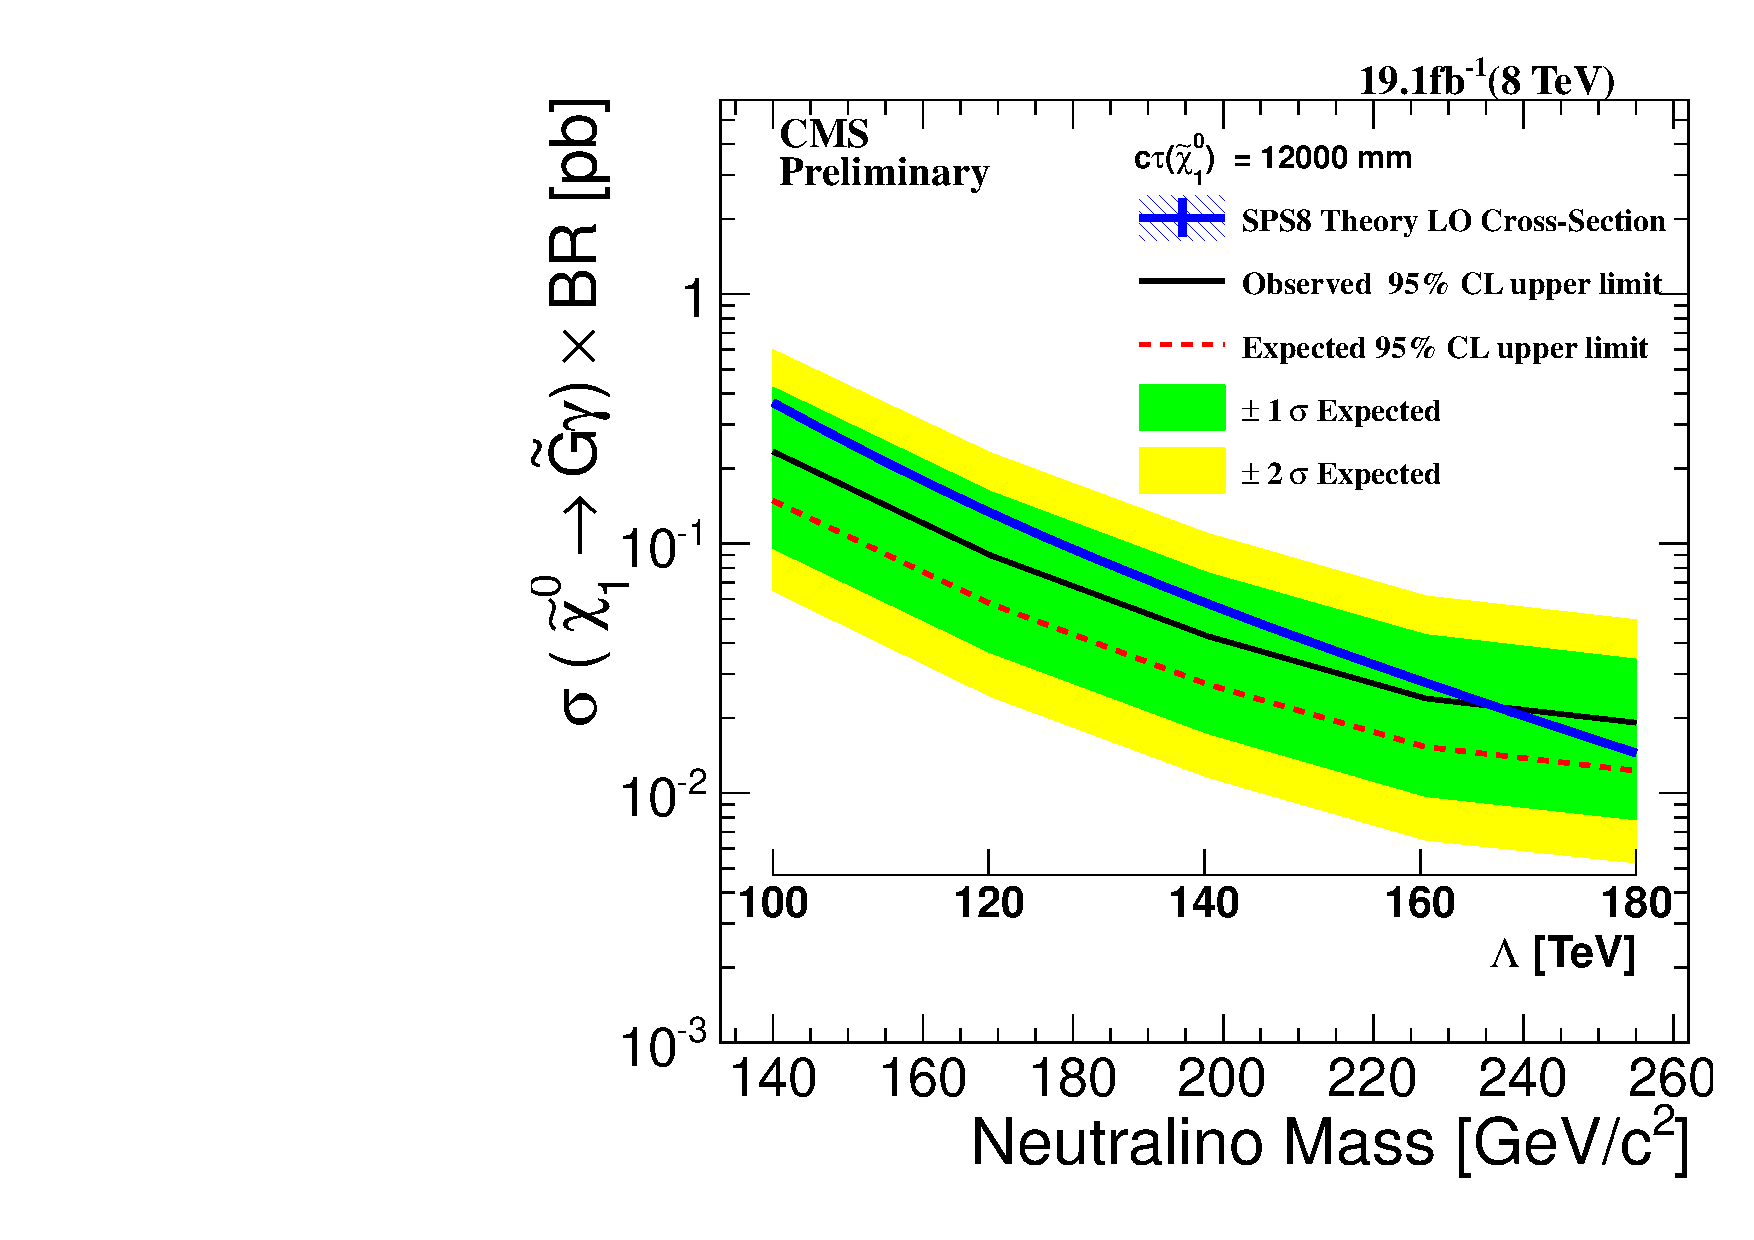
\includegraphics[height=6cm, width=\textwidth]{THESISPLOTS/Neutralino_CrosSecVsMass_Exclusion_limit_12000.pdf}}
\vspace{-1cm}
\caption{Mass Limit }
\label{fig:masslimit}
\end{minipage}
\end{figure}
\vspace{-1cm}
\alert{\textbf{sample is $c\tau= 12000$ mm but we measure $c\tau \approx 10500$ mm}}
\end{frame}

\begin{frame}
\frametitle{\Huge{$c\tau$-Mass Limits}}
 \begin{minipage}[t]{0.8\linewidth}
 %    \centering
      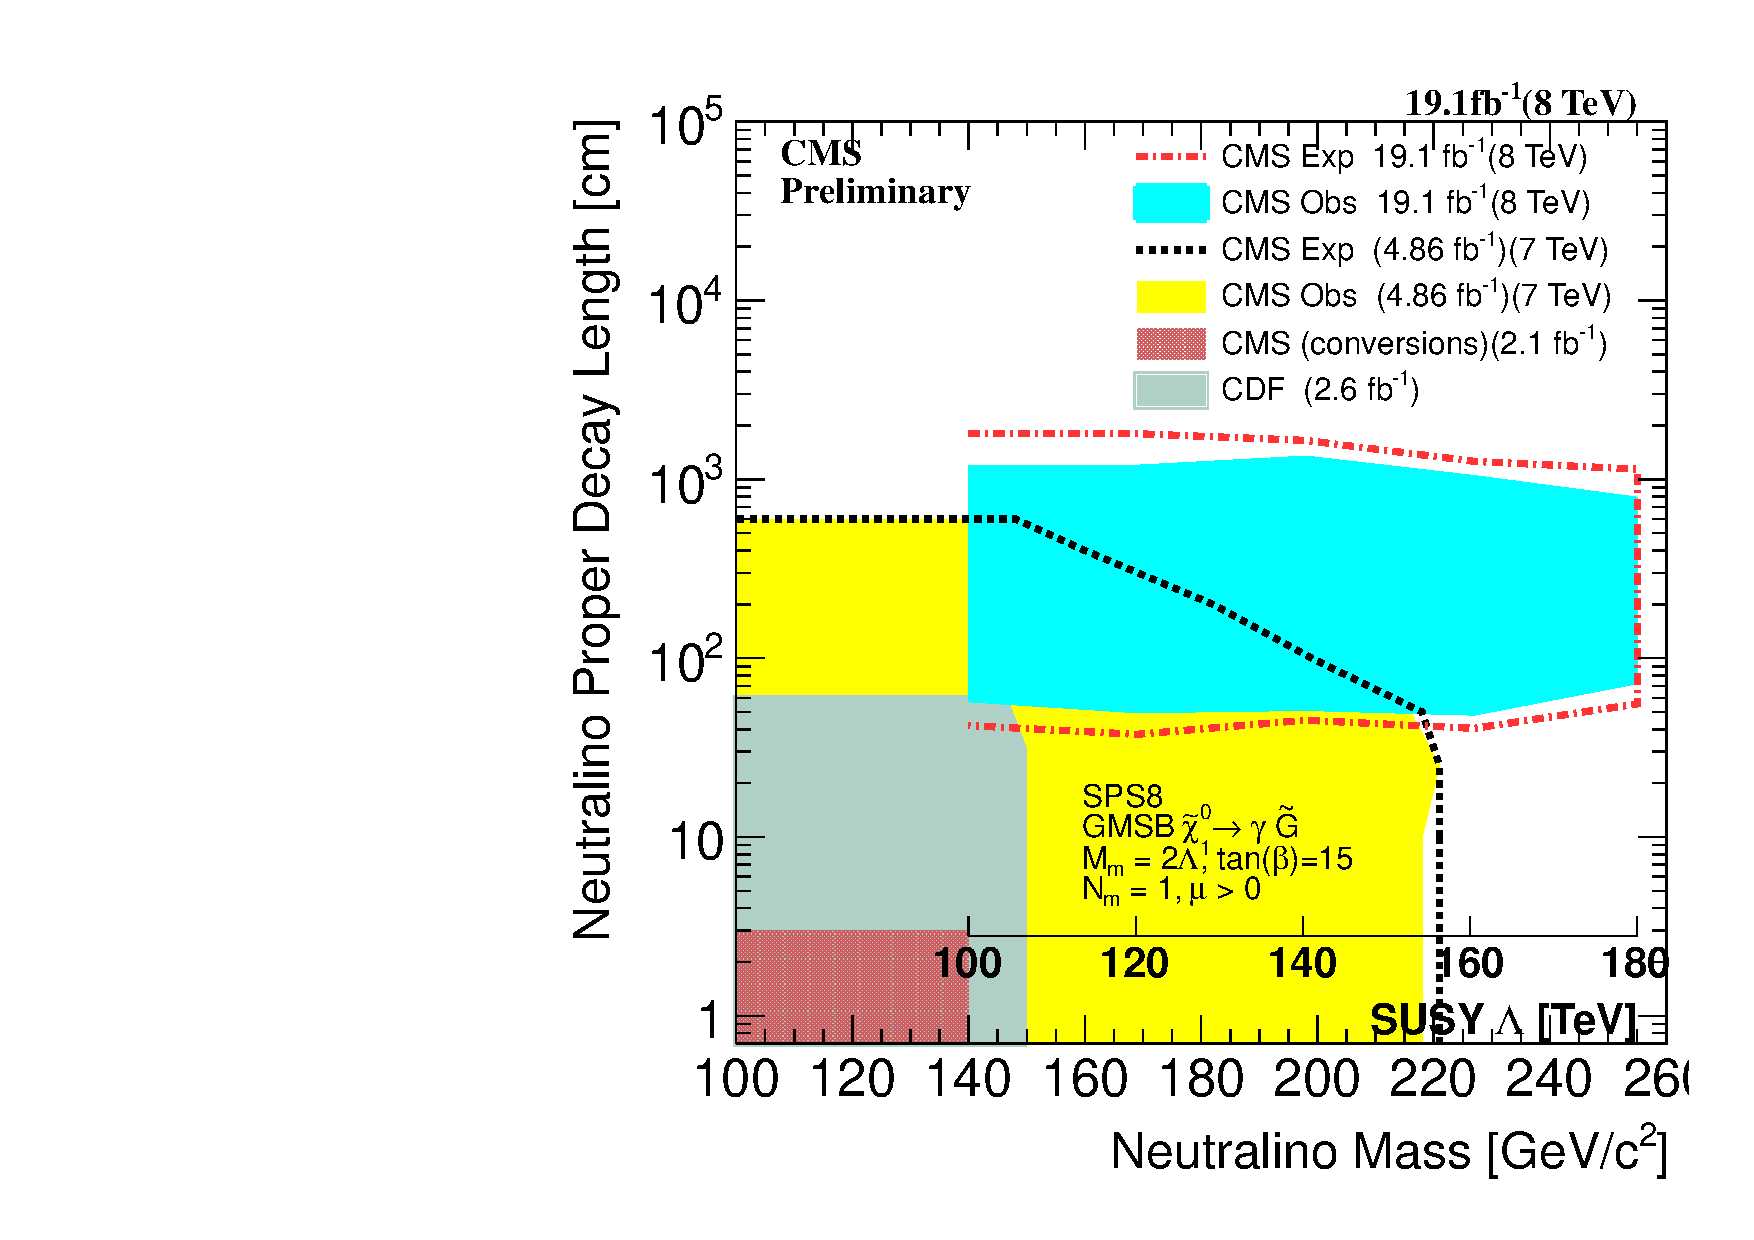
\includegraphics[height= 8cm,width=0.8\paperwidth]{THESISPLOTS/Neutralino_Ctau-Vs-Lambda_2D_exclusion.pdf}
%   \end{minipage}
% \begin{minipage}[t]{\linewidth}
% \newline \textcolor{blue} {\texttt{Y. Kats et al: arXiv:1110.6444v2}}
 \end{minipage}
\end{frame}



%others
%\begin{frame} %---------------------------------------------------------------
%\frametitle{Are these measurements correct?}
% \framesubtitle{}
%\begin{LARGE}
%\textbf{Are we measuring the original $c\tau$ of the neutralino?}
%\end{LARGE}
%\vspace{-0.5cm}
%\begin{table}
%\begin{minipage}[b]{1.0\linewidth}
%\centering
%\begin{tabular}{|l||l||l||l|l|l|}
%\hline
%\multicolumn{5}{|c|}{\bfseries{CMS Official GMSB Samples}} \\
%\hline
%\bfseries{$\Lambda$[TeV]} & \bfseries{mass[GeV]} & \bfseries{$C_{grav}$} & \bfseries{c$\tau$[mm]} & \bfseries{Fit Value[mm]} \\
%\hline
%120 & 169 & 93.5 & 1000 & 657.89 \\
%120 & 169 & 162 & 3000 &1942.12 \\
%\hline
%\hline
%140 & 198 & 162 & 3000 & 1550.38 \\
%140 & 198 & 187 & 4000 & 2064.83 \\
%140 & 198 & 229 & 6000 & 3083.56 \\
%\hline
%\hline
%180 & 256 & 93.5 & 1000 & 378.64 \\
%180 & 256 & 132 & 2000 & 749.45 \\
%180 & 256 & 162 & 3000 & 1104.85 \\
%180 & 256 & 229 & 6000 & 2203.61 \\
%\hline
%\end{tabular}
%\end{minipage}
%\end{table}
%\vspace{-0.5cm}
%\alert{\textbf{We seem to be measuring neutralino $c\tau$ by some factor off.}}
%\end{frame}
%\begin{frame}
%--------------------------------------------------------------------
%\frametitle{GMSB Sample $c\tau$ Vs Measured $c\tau$}
%\begin{LARGE}
%\textbf{By how much are we off in neutralino $c\tau$ measurements?}
%\end{LARGE}
%\begin{table}
%\begin{minipage}[b]{1.0\linewidth}
%\centering
%\begin{tabular}{|l||l||l||l|}
%\hline
%\multicolumn{4}{|c|}{\bfseries{CMS Official GMSB Samples}} \\
%\hline
%\bfseries{$\Lambda$[TeV]} & \bfseries{c$\tau$[mm]} & \bfseries{Fit Value[mm]} &\bfseries{Factor Off} \\
%\hline
%120 & 3000 & 1942.12 & 1.54 \\
%140 & 3000 & 1550.38 & 1.93 \\
%180 & 3000 & 1104.85 & 2.71 \\
%\hline
%\hline
%140 & 6000 & 3083.56 & 1.9 \\
%180 & 6000 & 2203..61 & 2.7 \\
%\hline
%\end{tabular}
%\end{minipage}
%\end{table}
%\vspace{-0.5cm}
%Factor is \alert{The SAME} for different neutralino $c\tau$ with same $\Lambda$ value. However, factor is \alert{NOT THE SAME} for the same $c\tau$ with different $\Lambda$ values.
%\end{frame}
%\begin{frame}
%---------------------------------------------------------------------
%\frametitle{Cause of this difference in $c\tau$ values?}
%\begin{LARGE}
%\textbf{Is this due to how sample is generated?}
%\end{LARGE}
%\vspace{-0.3cm}
%\begin{figure}[ht]
%\begin{minipage}[b]{0.45\linewidth}
%\centering
%\mbox{
%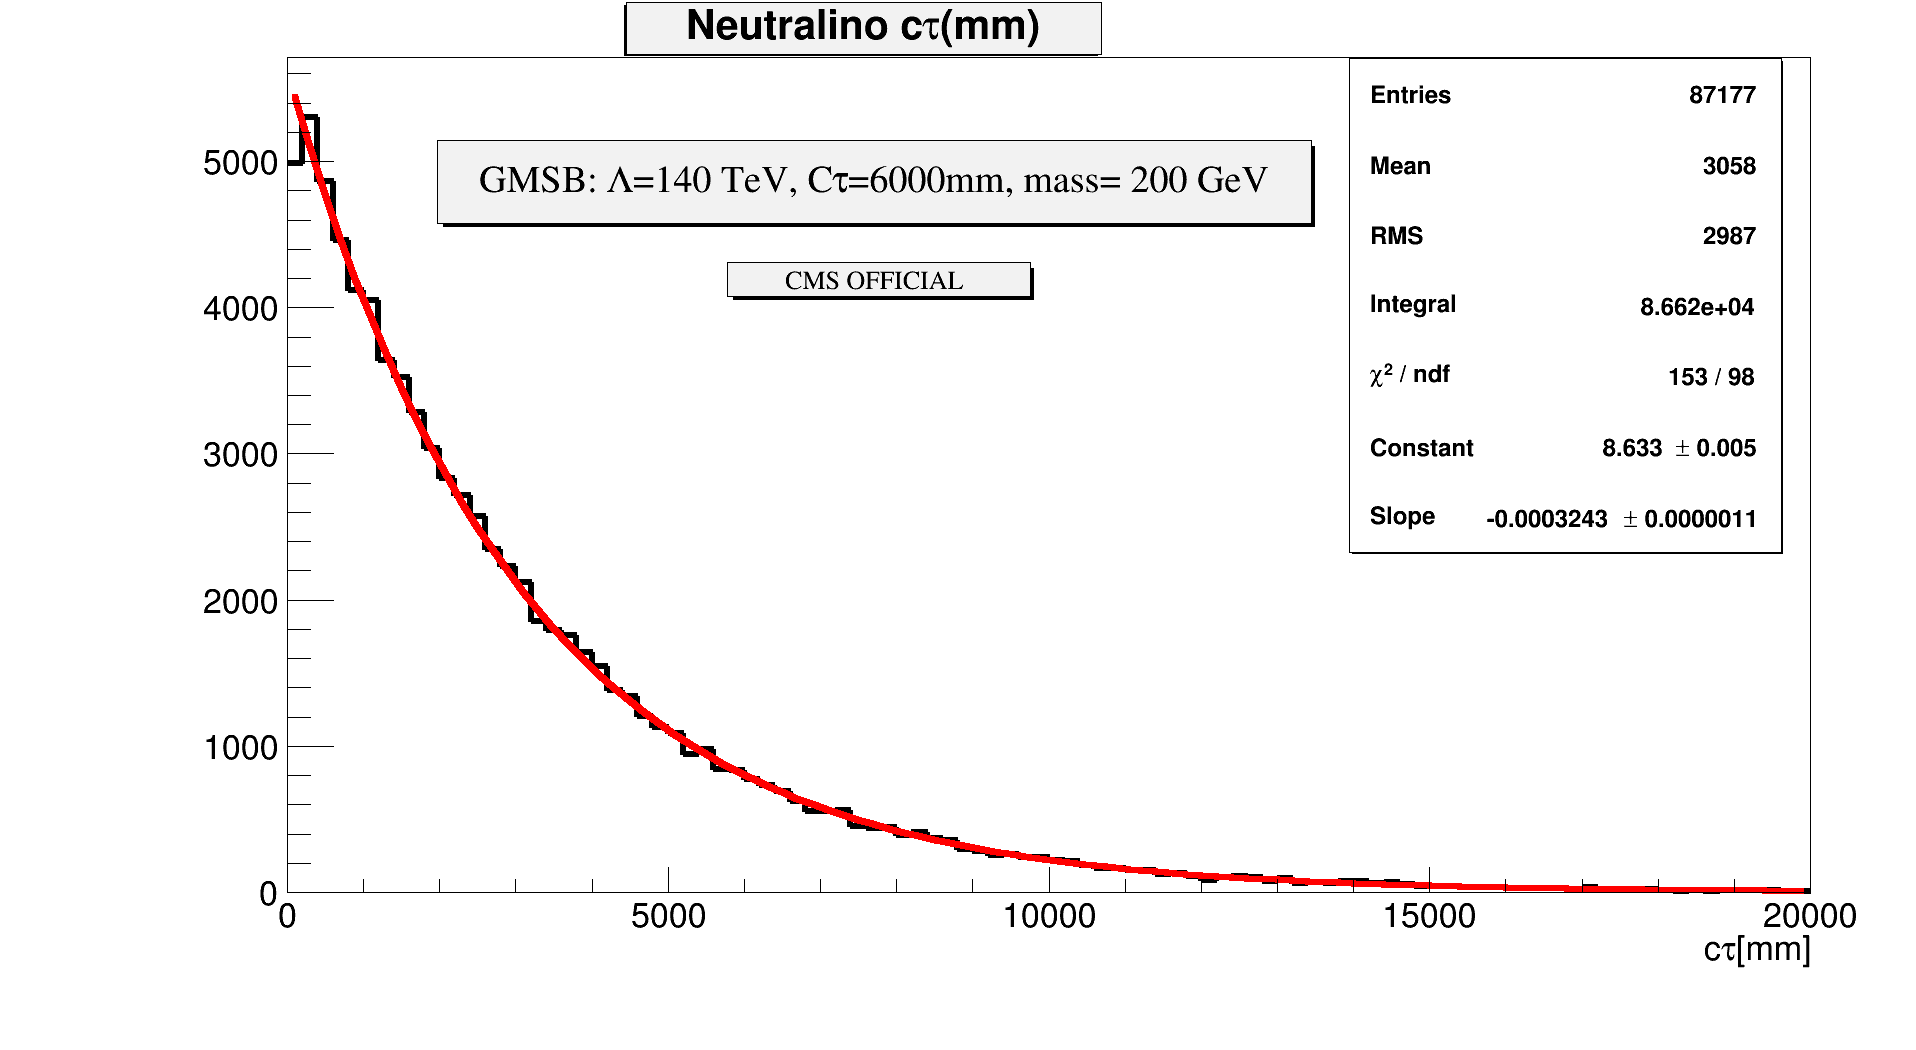
\includegraphics[height=2.5cm, width=\textwidth]{MC_TimeDL.png}}
%\vspace{-1cm}
%\caption{1/Slope = 3083.56 mm }
%\label{fig:OffFrom_MC}
%\end{minipage}
%\hspace{0.1cm}
%\begin{minipage}[b]{0.45\linewidth}
%\centering
%\mbox{
%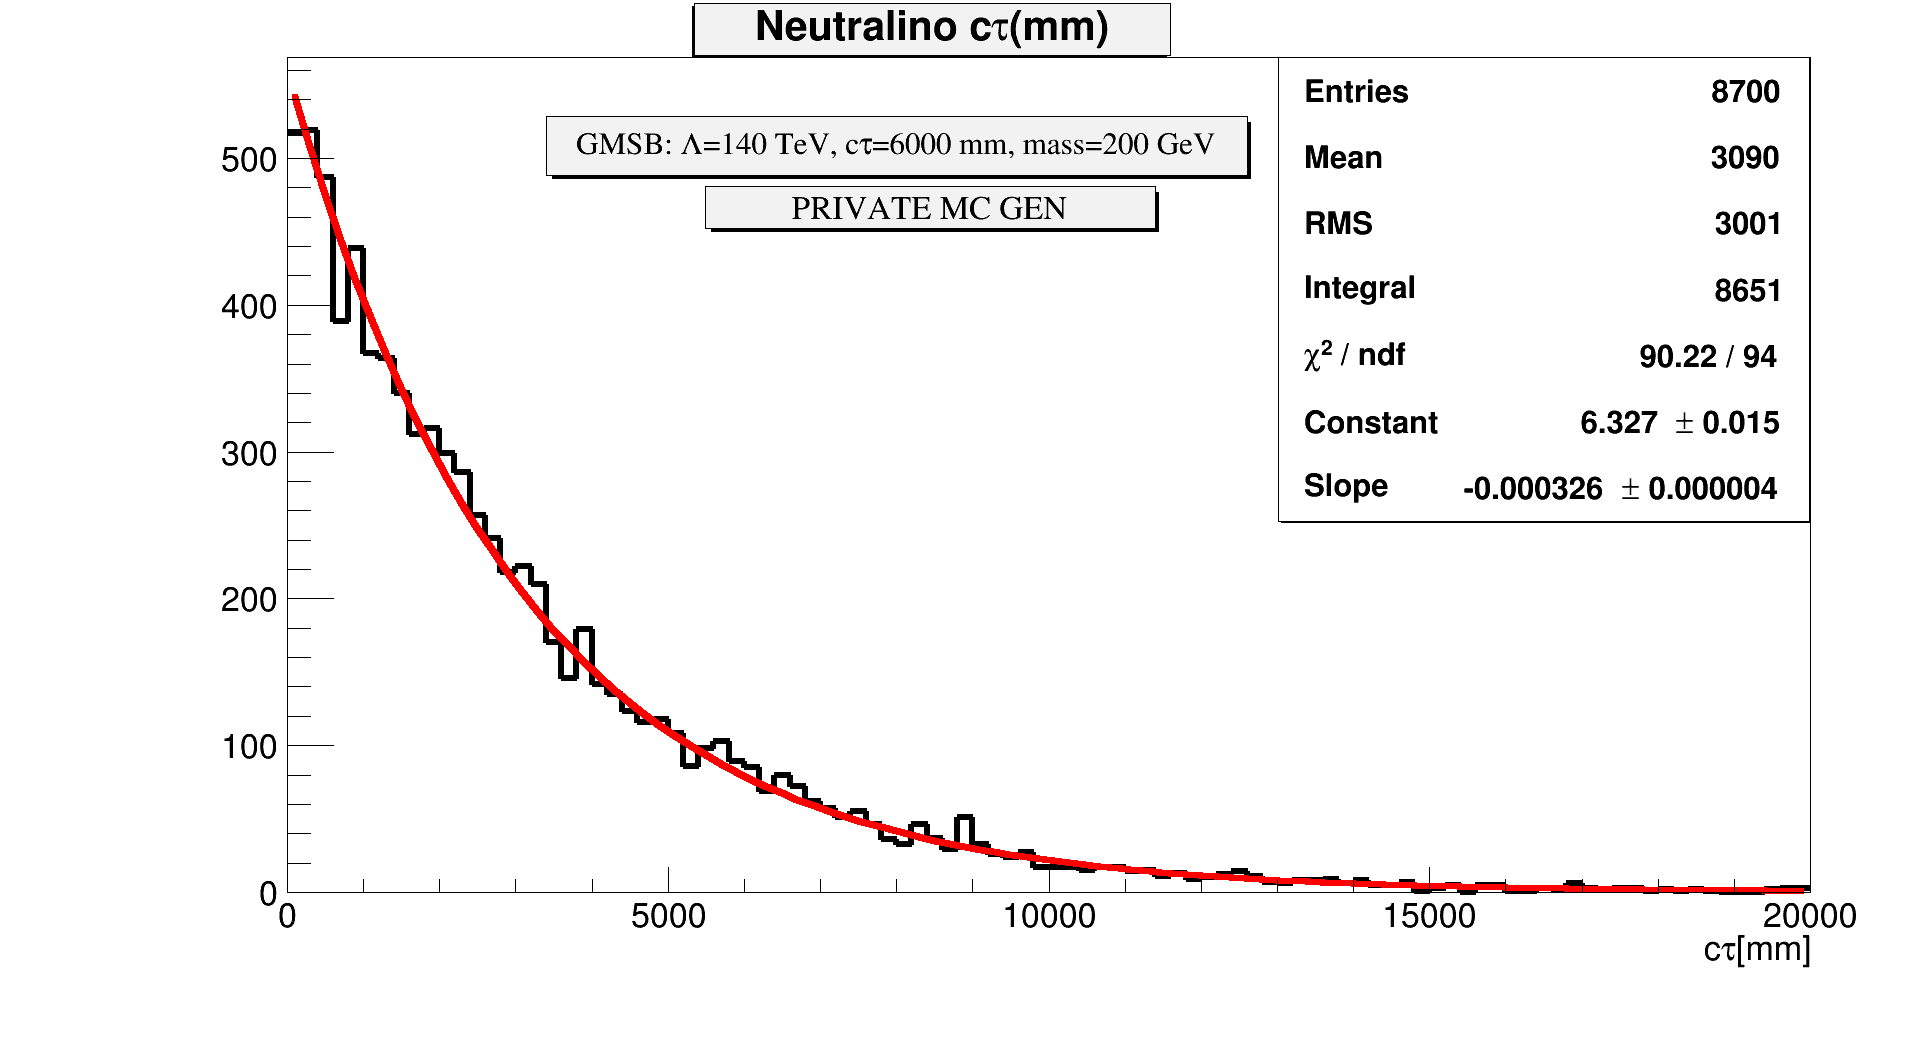
\includegraphics[height=2.5cm,width=\textwidth]{Priv_MC_TimeDL.png}}
%\vspace{-1cm}
%\caption{1/Slope = 3067.48 mm }
%\label{fig:Priv_MCTime}
%\end{minipage}
%\end{figure}
%\vspace{-1.0cm}
%\begin{figure}[ht]
%\begin{minipage}[b]{0.45\linewidth}
%\centering
%\mbox{
%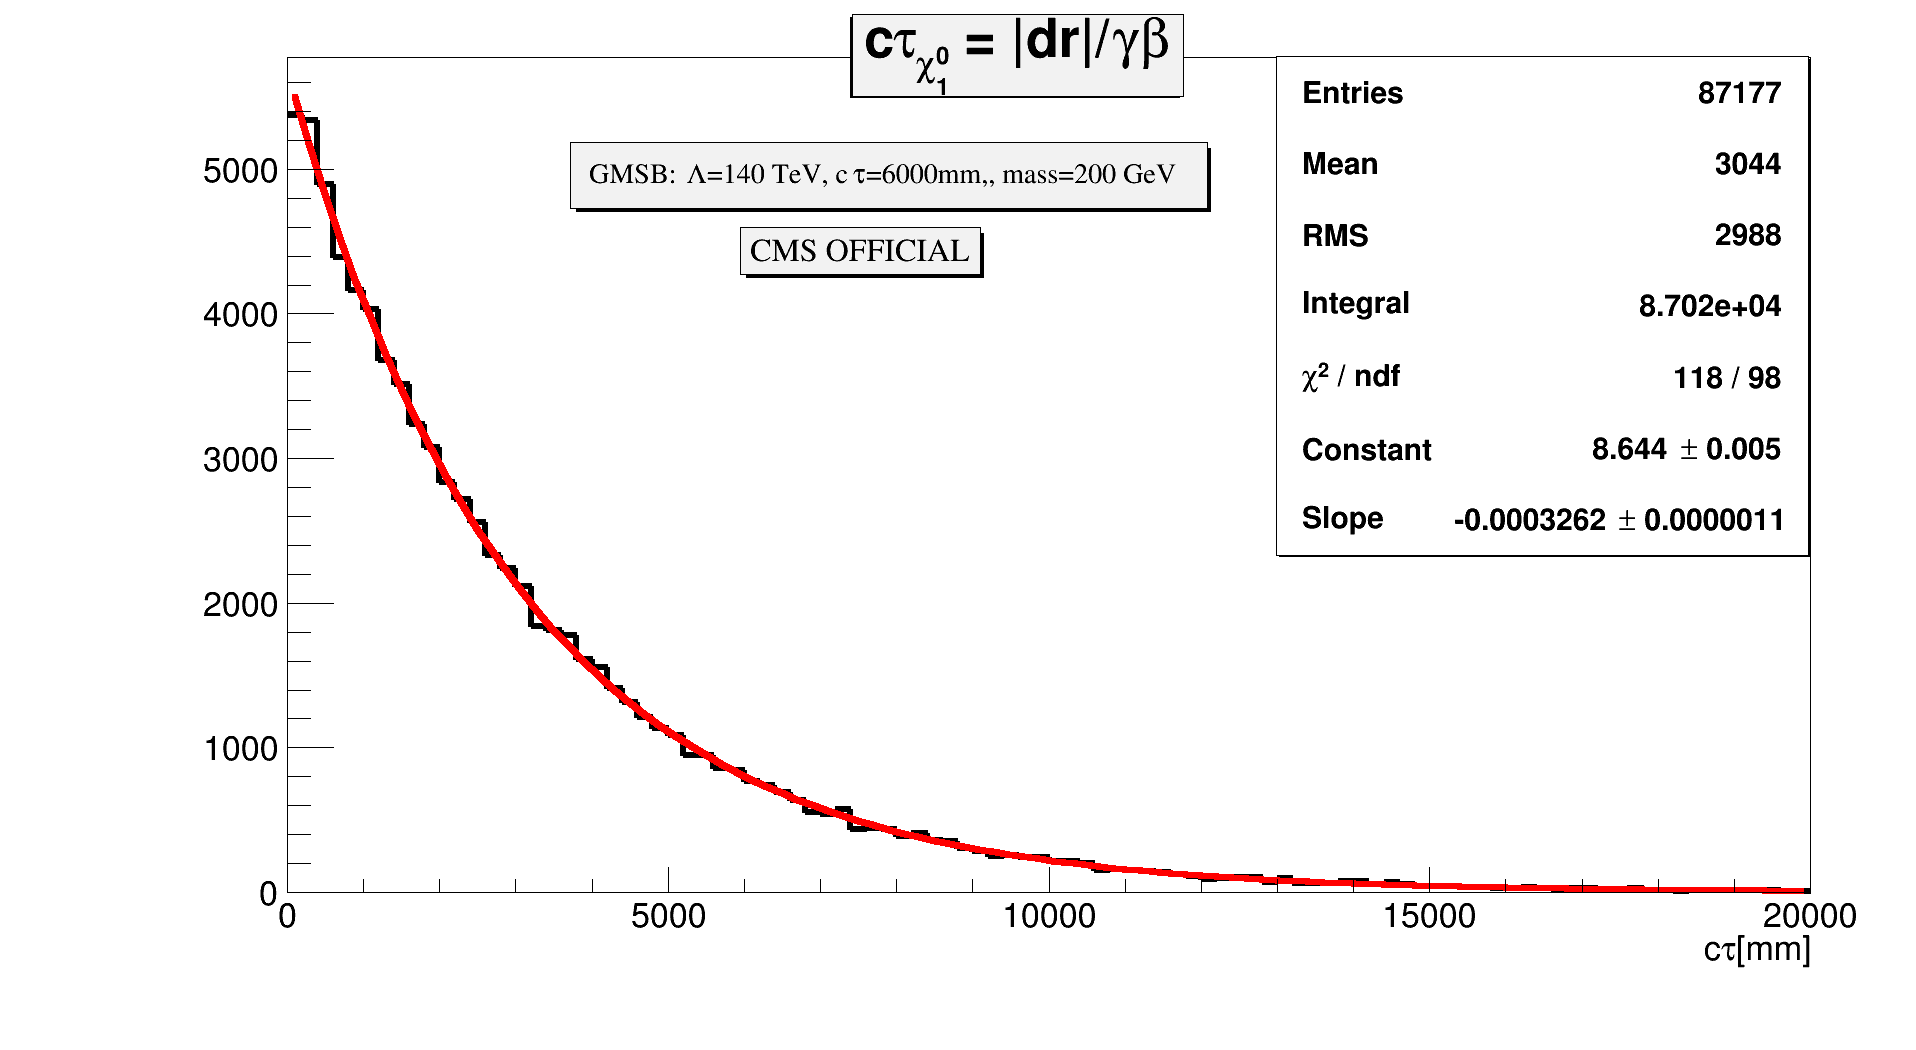
\includegraphics[height=2.5cm, width=\textwidth]{Dist_TravDL.png}}
%\vspace{-1cm}
%\caption{1/Slope = 3065.60 mm }
%\label{fig:Off_DL}
%\end{minipage}
%\hspace{0.1cm}
%\begin{minipage}[b]{0.45\linewidth}
%\centering
%\mbox{
%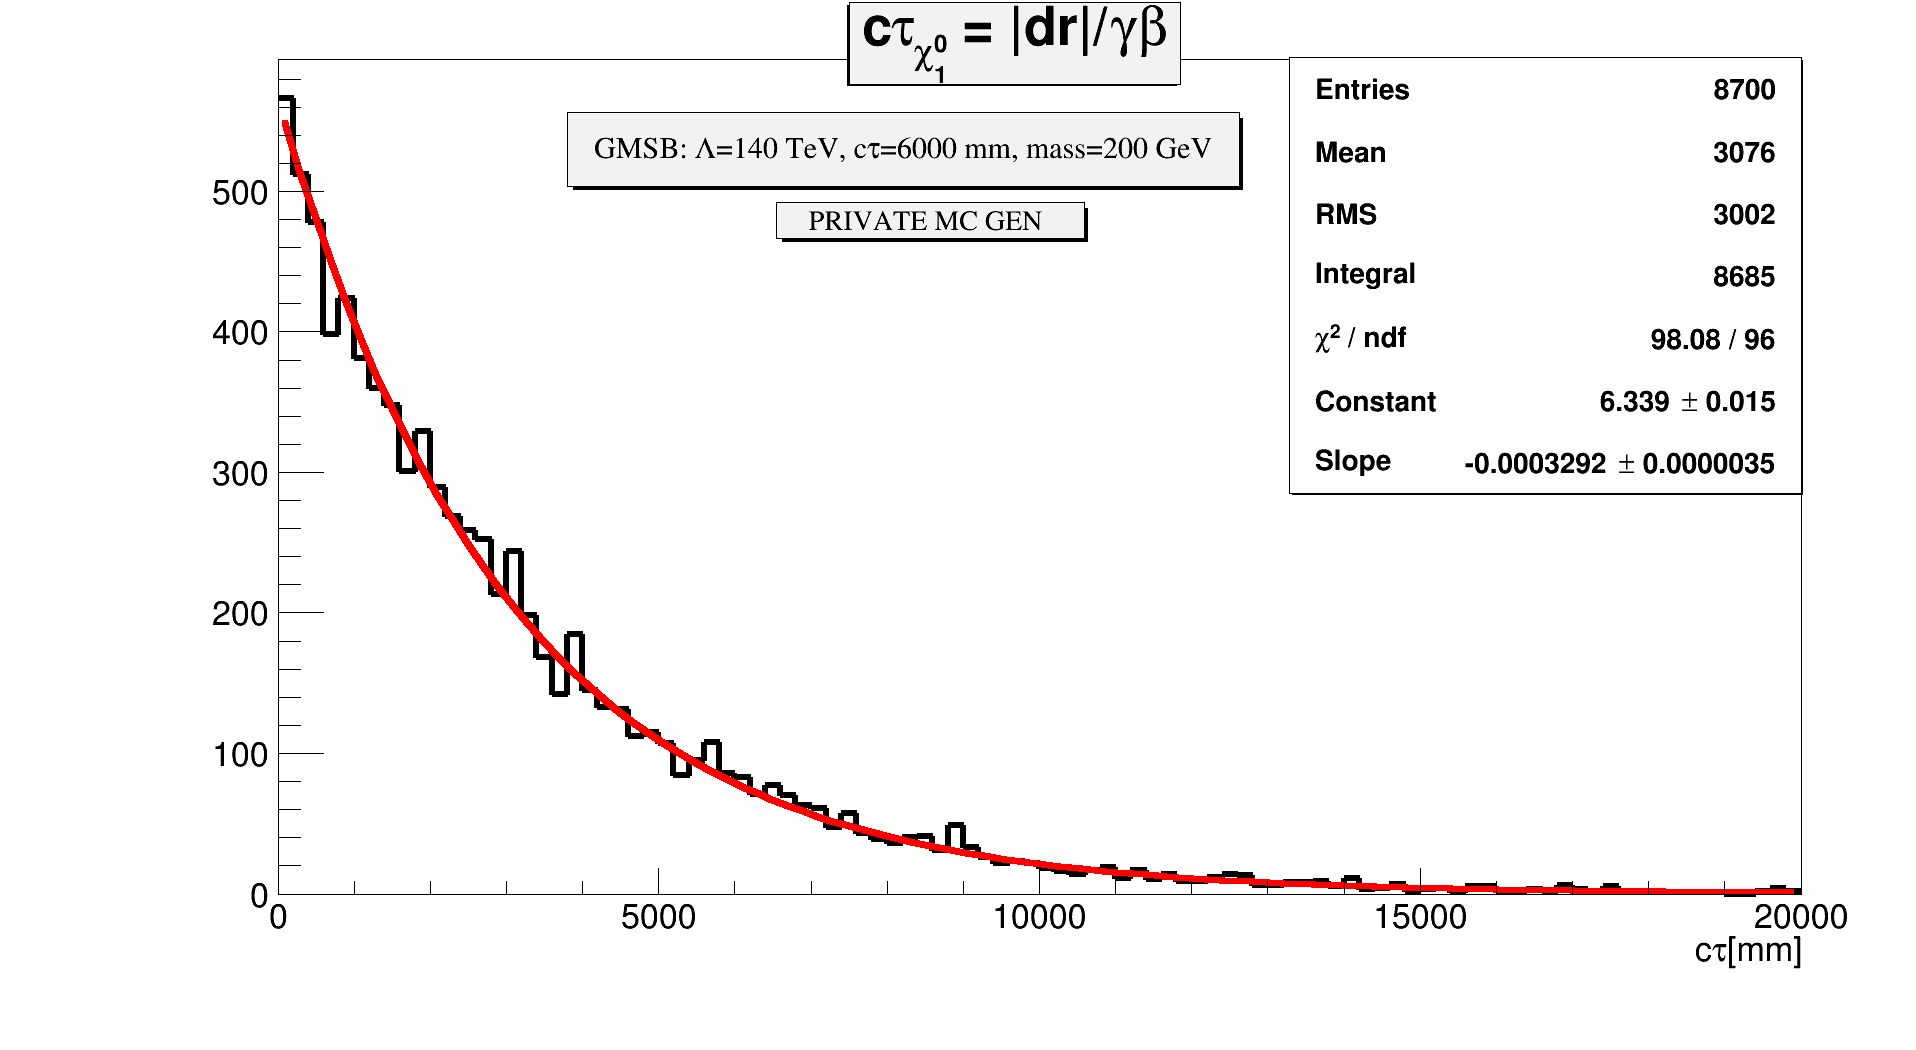
\includegraphics[height=2.5cm,width=\textwidth]{Priv_DistTravDL.png}}
%\vspace{-1cm}
%\caption{1/Slope = 3037.66 mm }
%\label{fig:Priv_DL}
%\end{minipage}
%\end{figure}
%\vspace{-1.0cm}
%\alert{\textit{Private GMSB sample seems to show same offset measurements}}
%\end{frame}
\section{Summary}
\begin{frame}
\frametitle{\Huge Summary}
%\begin{itemize}
%\begin{large}
%\item Offset in neutralino $c\tau$ seems to have a more subtle origin than expected. Probably how mass enters into the lifetime definition and implementation at MC generation level.
%\item GMSB samples with the same sample $c\tau$, hence $C_{grav}$, but with different $\Lambda$ values have different offset factor.
%\item The observation that the $c\tau$ value for a given sample with $\Lambda$ is different from the measured value is very unclear, even without looking at samples with different $\Lambda$ values.
%\item Our next step involves understanding cause of this offset.
%However,due to time constraints, we might continue with upper limit setting considering this difference.
%\end{large}
%\end{itemize}
\end{frame}
\end{document}
%\begin{frame}
%\frametitle{Introduction}
%\begin{varblock}[7cm]{Hybrid Linear Modeling}
%Suppose $\textbf{X} = \left( \mathbf{x}_{1}, \cdots, \mathbf{x}_{N} \right)$.
%sampled from a mixture of $\kappa$ subspaces or flats with dimension $d$
%\end{varblock}
%\begin{itemize}
%\item Assumptions:
%\end{itemize}
%\end{frame}

